\chapter{Empirical Evaluation}\label{chap:4}
\section{Available data description}
Pabutools library contains hundreds of historical, real-life instances of participatory budgeting elections, from numerous Polish cities such as Warsaw, Częstochowa, Poznań, Gdańsk and more. Elections contain both city-wide vote profiles, as well as profiles specific for cities' districts. Elections vary greatly in size, with the number of voters ranging from less than $100$ to over $100,000$ with over $200$ projects available.

Most of the available instances are approval-based elections. However, we treat them as if cardinal ballots were cast, where the utility from a supported project is equal to its cost, that is we use cost satisfaction measure. A minority of instances allow for \emph{cumulative ballots}, which are cardinal profiles with additional constraints. Voters are allowed to split some number of points among projects, with minimal and maximal number of points being assignable to a single candidate. Also a small group of instances are ordinal-based elections, where voters sort the projects by their preference. Because stable priceability is not defined for this type of ballots, we do not evaluate our work on these instances.

In total, we analyse $96$ instances of elections with cumulative profiles and $398$ elections with approval profiles. The instances were selected from the Pabulib library in ascending order of the product $(\text{number of voters})\cdot(\text{number of projects})$, as this is the factor defining the size of the linear program. Some of the larger instances in the repository have been omitted due to computational constraints. As problem size increases, solver runtime grows rapidly. We therefore imposed a fixed wall-clock limit and excluded instances exceeding it.  In the next sections, we test different voting rules and check their effectiveness in finding priceable and stable-priceable outcomes, as well as look at how often exhaustive outcomes prove to be stable-priceable.

All scripts used to process the election data, run the experiments and generate the results presented in this chapter are available in a public repository~\cite{Chapter4Scripts}.
\section{Existence of stable-priceable allocations}
We consider the following election rules:
\begin{itemize}
    \item MES --- the classic Method of Equal Shares
    \item MES+BOS --- MES with Bounded Overspending
    \item MES+Inc --- MES with voter budget increment
    \item MES+Inc+UGreedy --- MES with voter budget increment and greedy fill
    \item UGreedy --- the classic utilitarian greedy method.
\end{itemize}
Firstly, we consider elections with cumulative profiles, with \emph{AdditiveCardinalSat} satisfaction measure. That is, a voter $i$'s satisfaction of the outcome $W$ is equal to the sum of scores assigned to $W\cap A(i)$.
\begin{figure}[H]         
  \centering              
  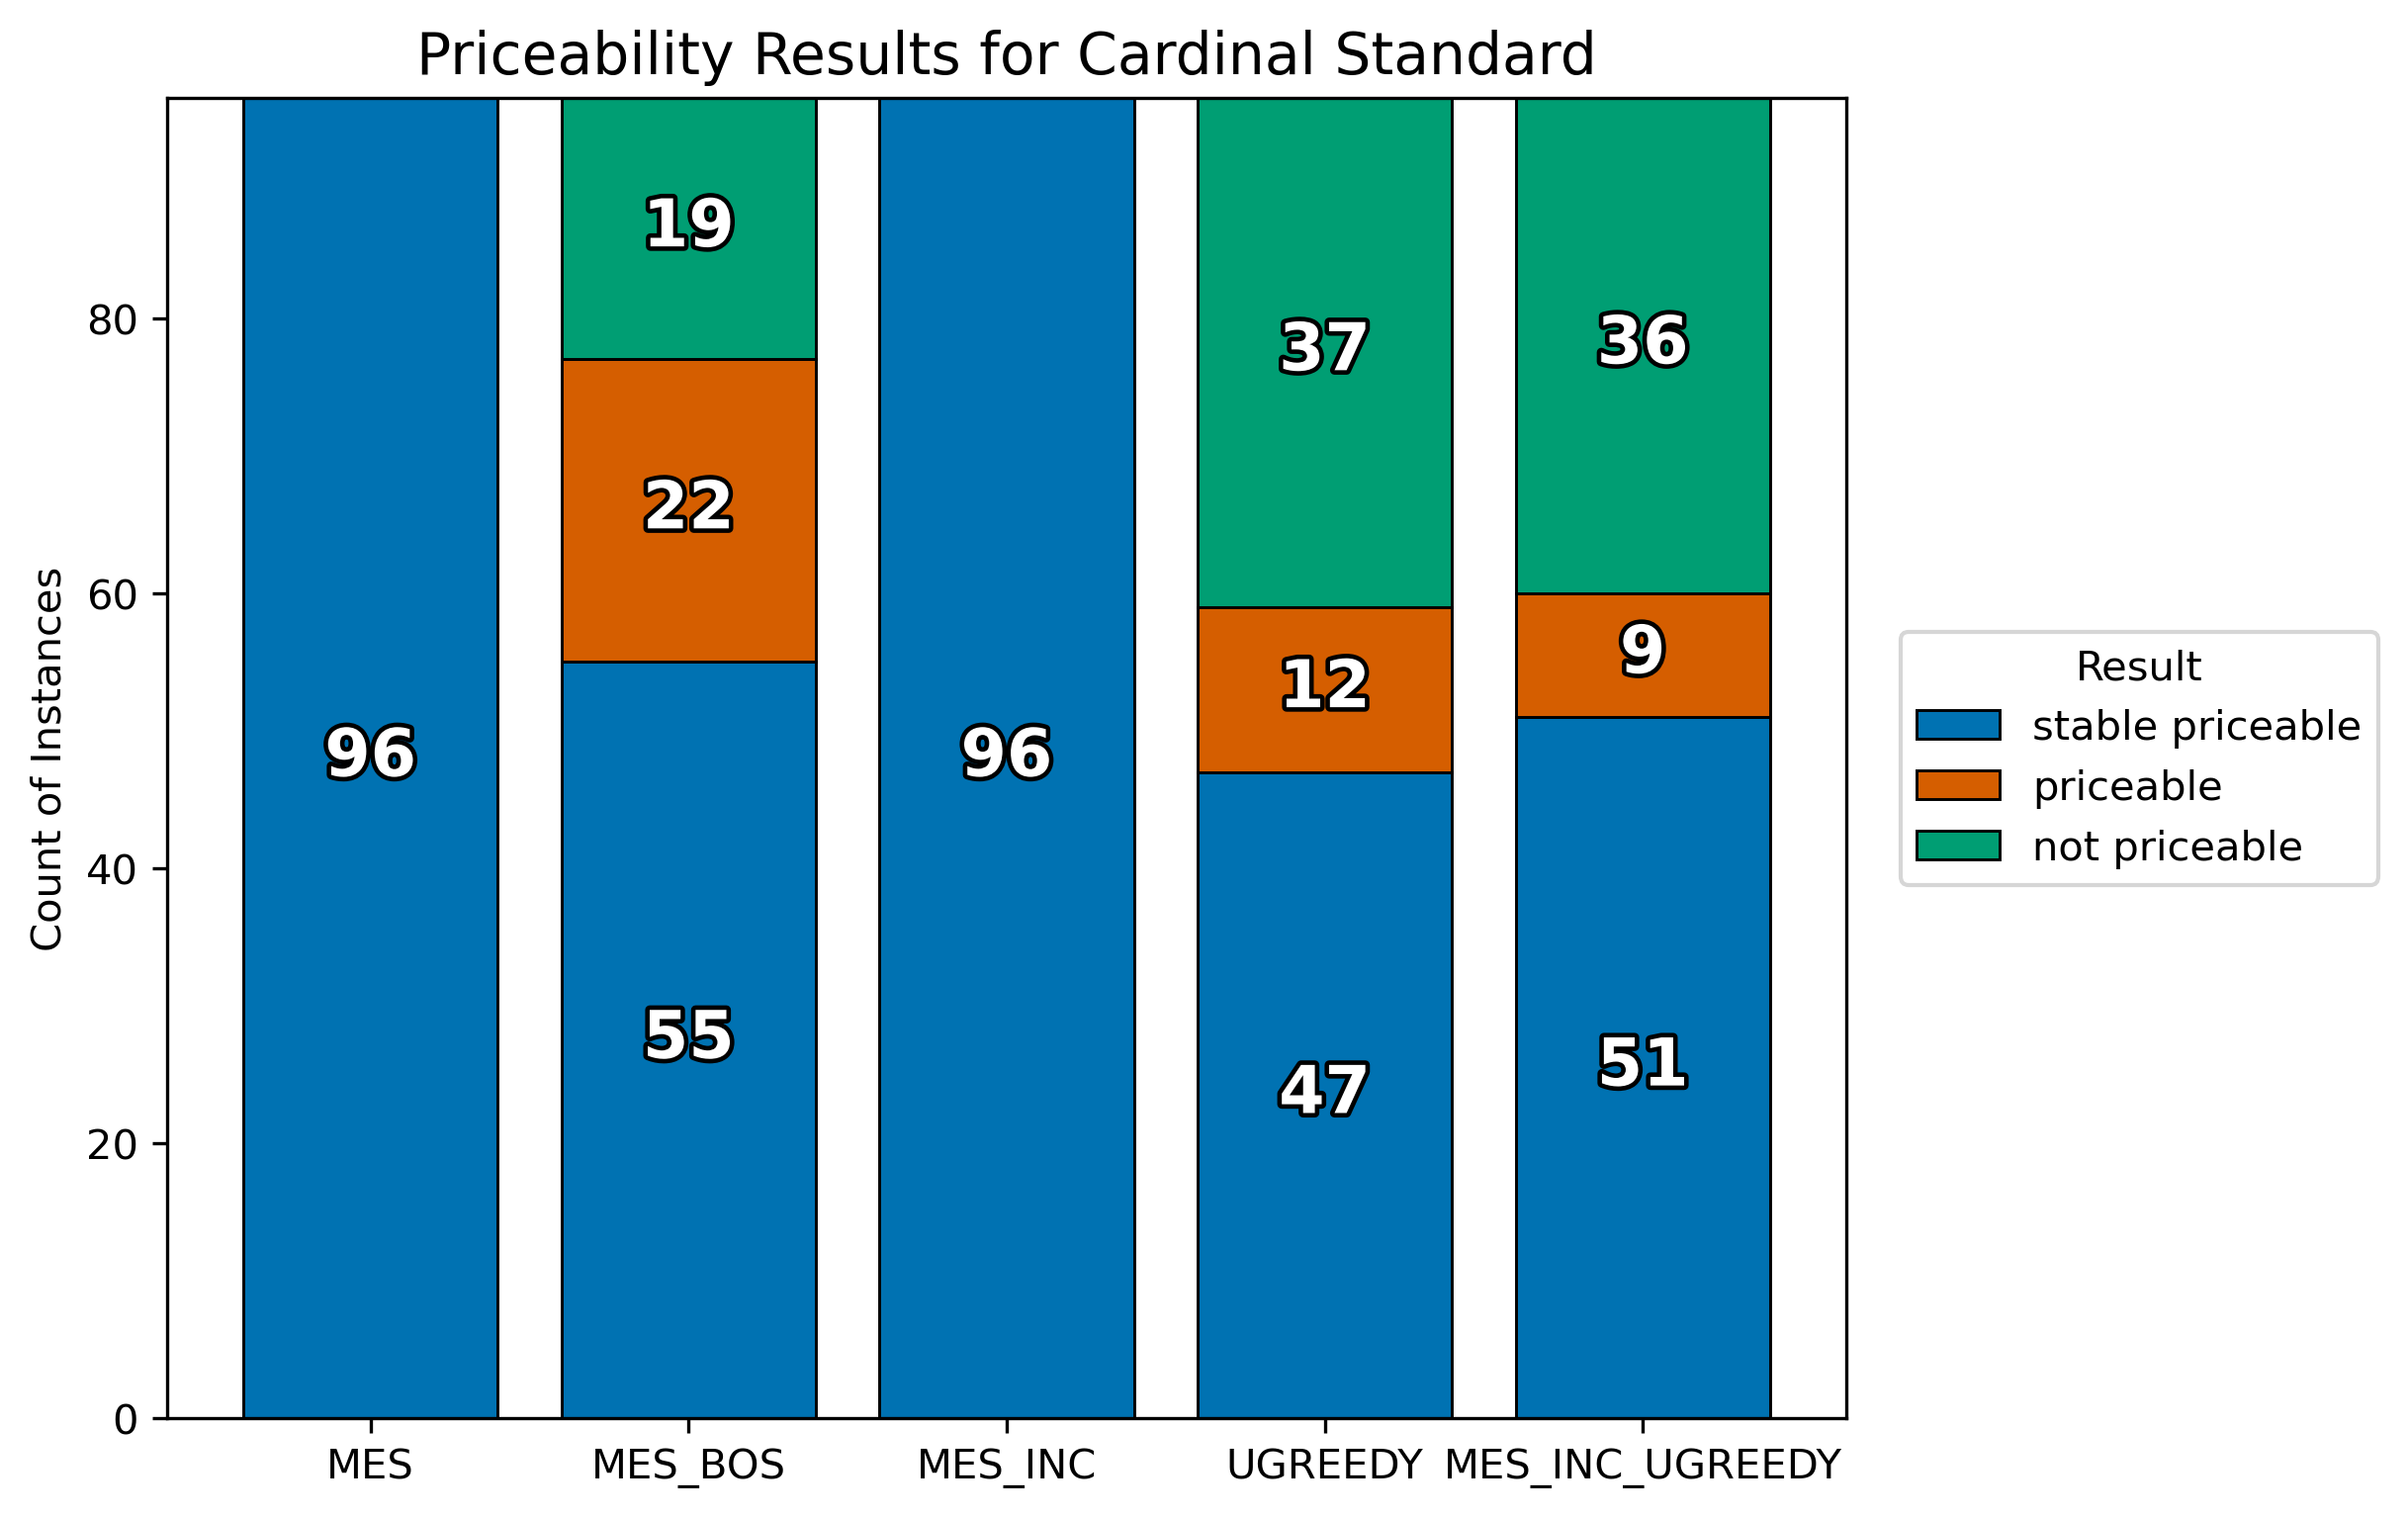
\includegraphics[width=0.7\textwidth]{figures/plots/cardinal-standard/cardinal_standard_priceability.png}
  \caption{Stable priceability and priceability of allocations returned by selected election rules for unmodified cardinal-based elections.}
  \label{fig:myplot}
\end{figure}
When considering untouched cardinal-based elections, we can observe that pure MES and Mes+Inc score perfect $100\%$ of the allocations being stable priceable. The utilitarian greedy method provides stable priceable allocations only in less than half of all instances, while the MES filled with utilitarian greedy scores in between, but closer to pure UGreedy. This is expected, as the MES is proved to select very fair outcomes when working with the additive score satisfaction measure. MES with Bounded Overspending provides similar results to MES with greedy fill.


We also consider both elections with approval profiles and cumulative profiles. However, we adjust them to \emph{cost satisfaction measure}. Satisfaction score for each voter $i$ from a project $p$ is equal to the utility assigned by voter $i$ to $p$ multiplied by its cost $score_i(p)=u_i(p)\cdot cost(p)$. This is believed to be more representative of actual voters' satisfaction, as larger project typically bring greater satisfaction to their supporters. Naturally, our updated notion of stable priceability allows such an evaluation. Previously, analysis only for approval-based instances was possible.
\begin{figure}[H]         
  \centering              
  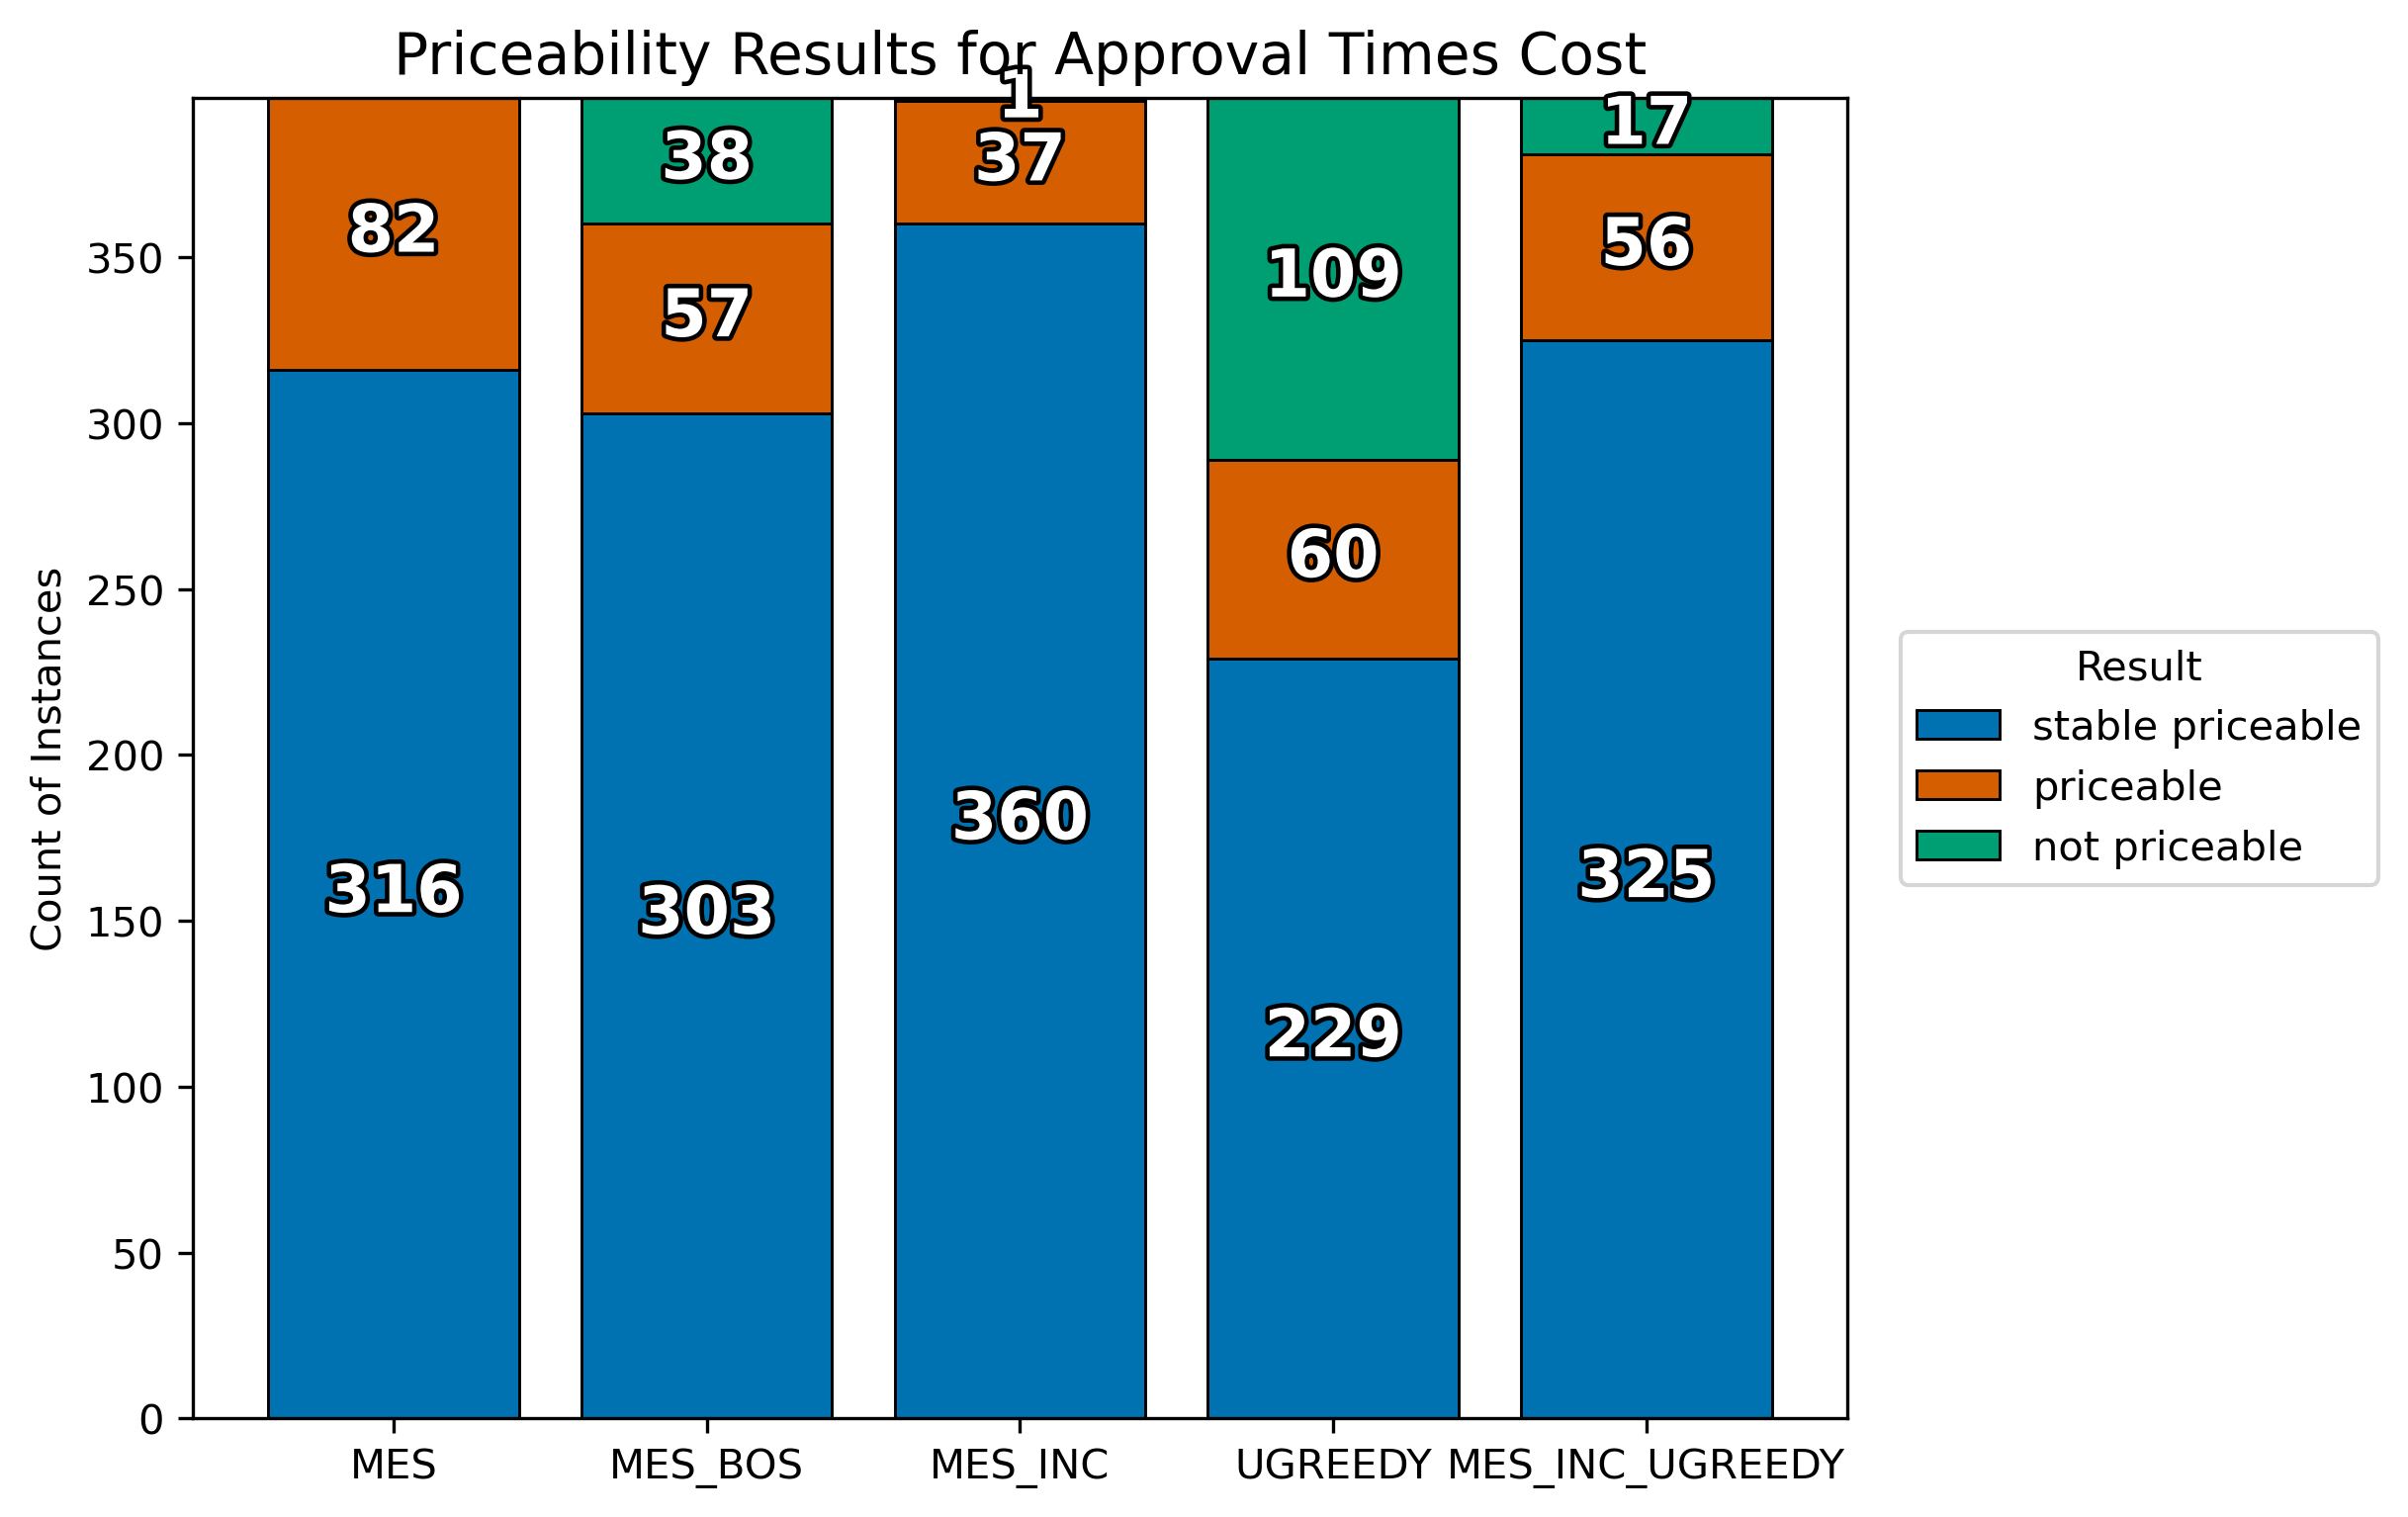
\includegraphics[width=0.7\textwidth]{figures/plots/approval-times-cost/approval_times_cost_priceability.png}
  \caption{Stable priceability and priceability of allocations returned by selected election rules for approval ballot instances multiplied by projects' costs.}
  \label{fig:myplot}
\end{figure}
As we can see from the plot above, the Utilitarian Greedy method performs by far the worst compared to variations of the Method of Equal Shares. Its primary aim of maximizing total voter utility often does not lead to returning proportional allocations. MES scores decently with around $79\%$ being stable priceable and the remainder priceable. Variation with voter budget increment does even better, with $90\%$ of stable priceable allocations. Again, filling MES allocations greedily until exhaustiveness affects priceability in a very negative way. BOS stands out the most for these instances, suggesting that it is more well-suited for cost satisfaction measure.
\begin{figure}[H]         
  \centering              
  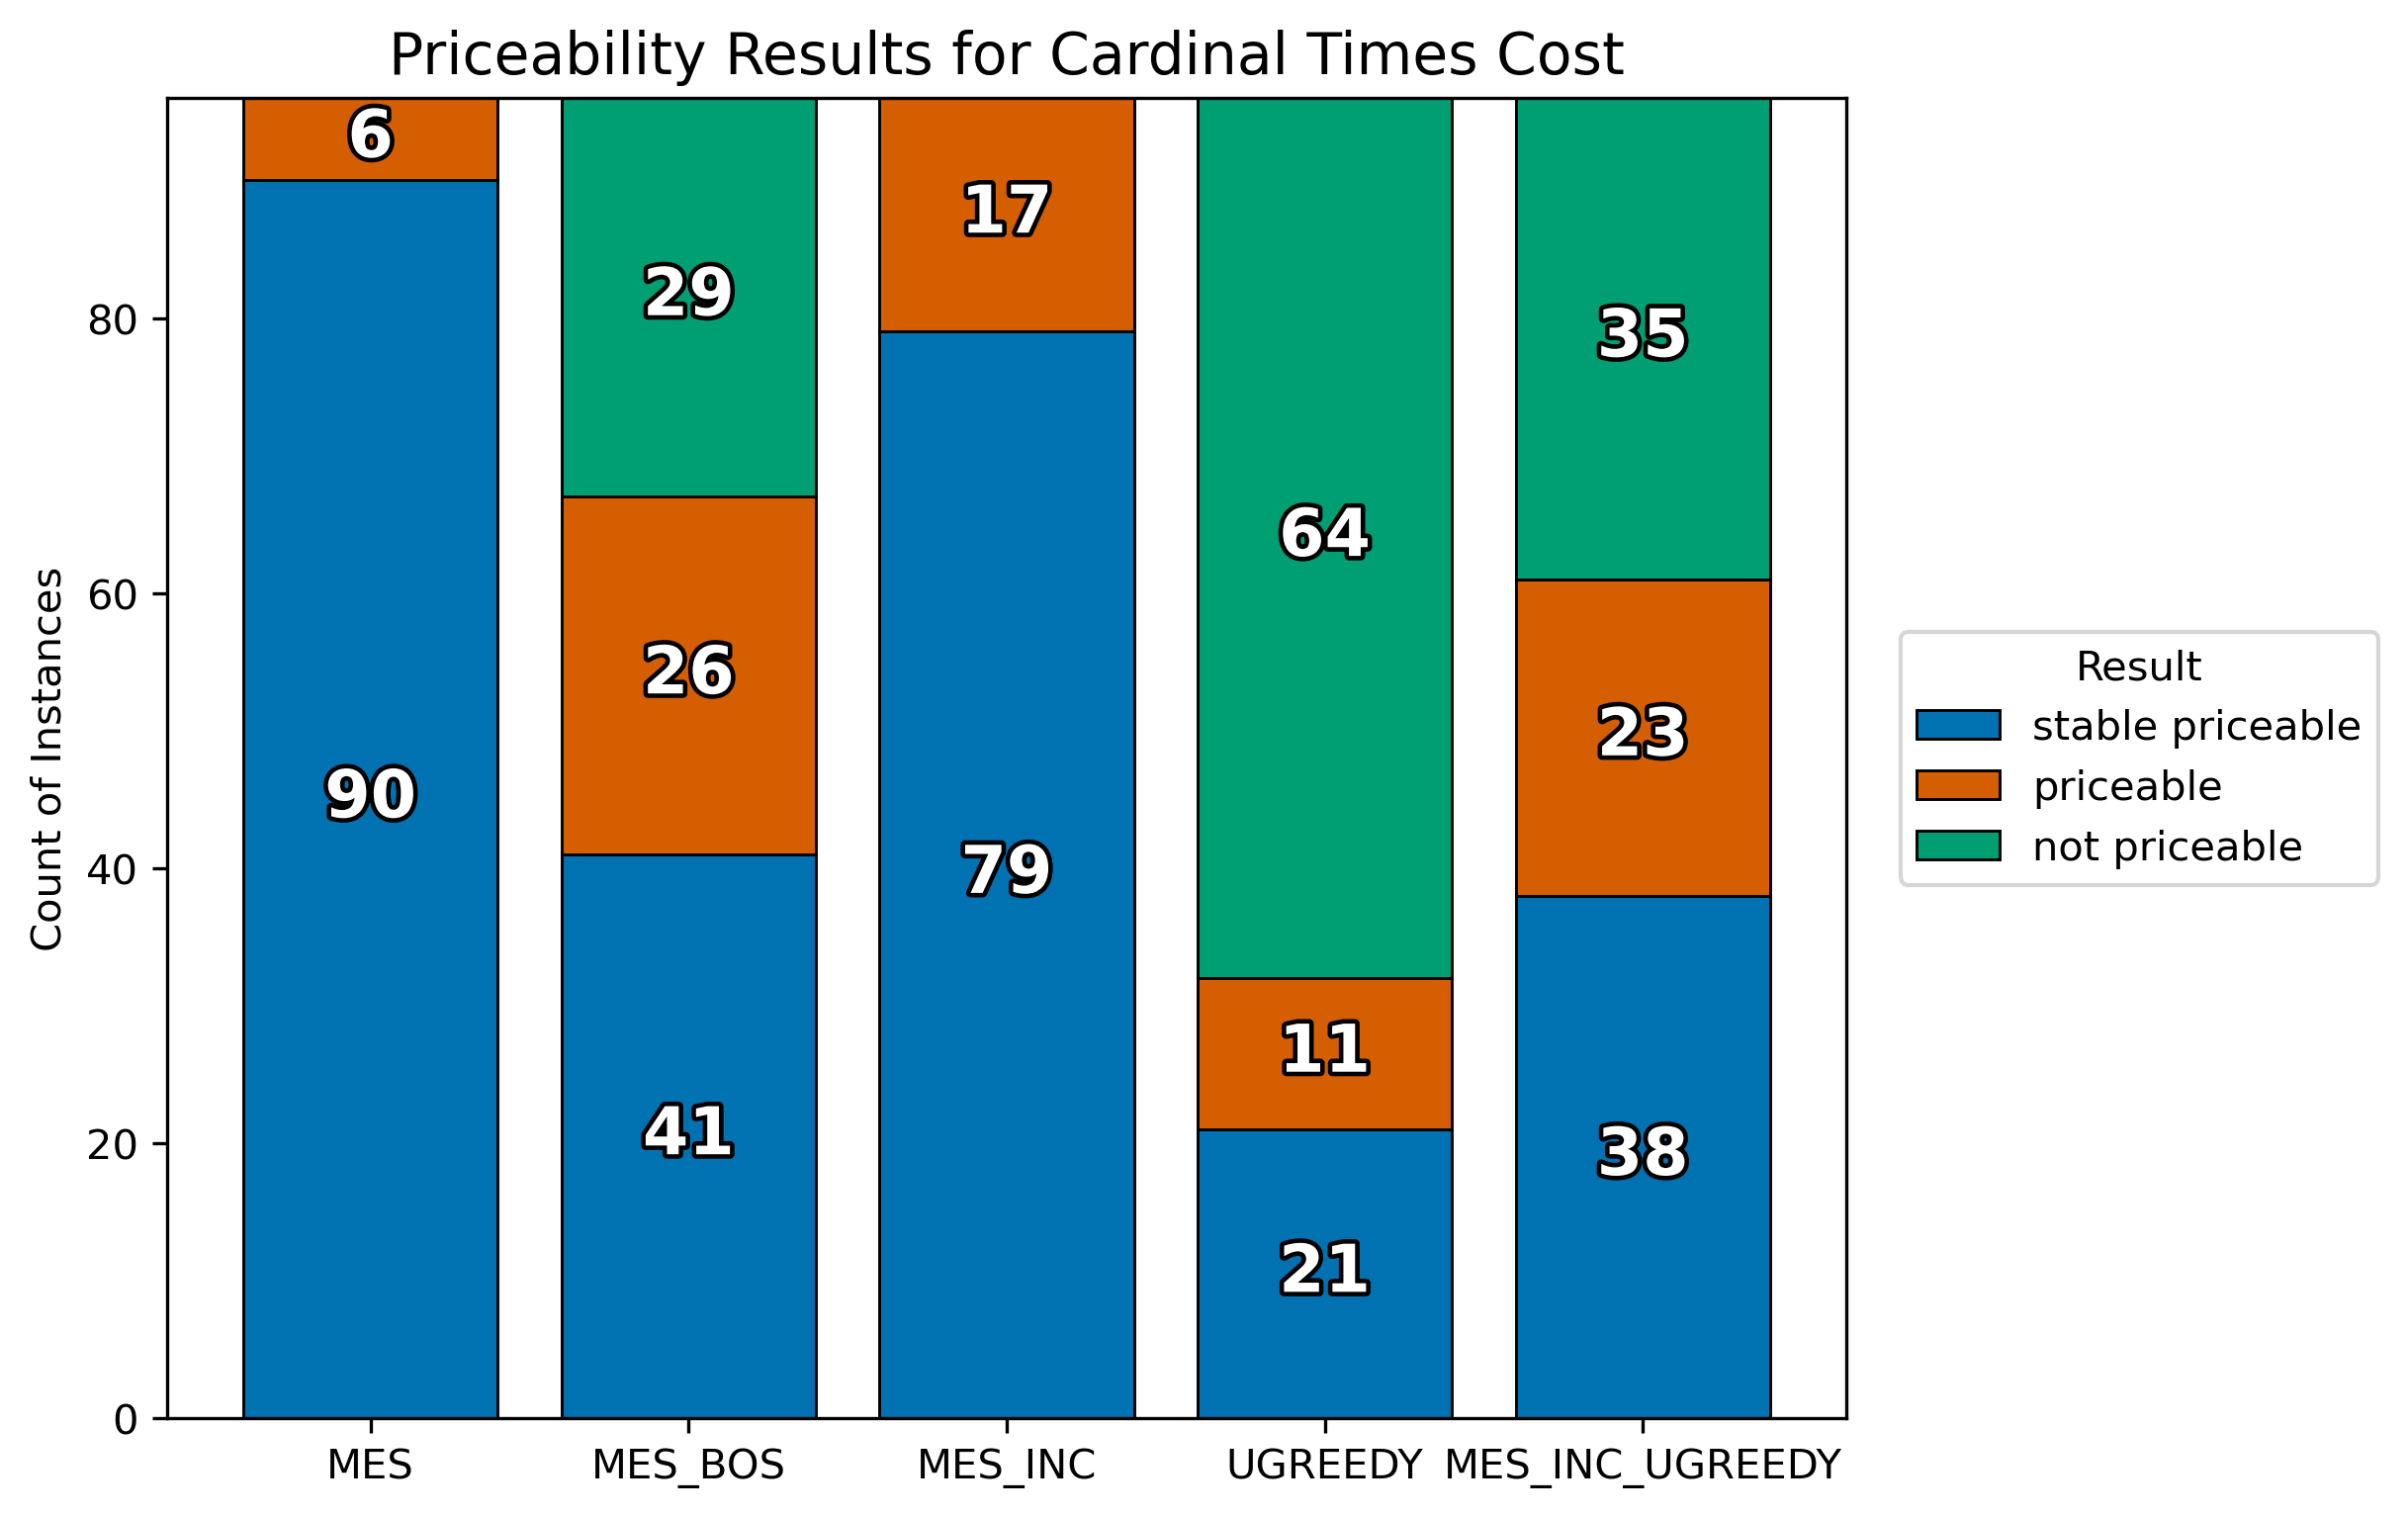
\includegraphics[width=0.7\textwidth]{figures/plots/cardinal-times-cost/cardinal_times_cost_priceability.png}
  \caption{Stable priceability and priceability of allocations returned by selected election rules for cardinal ballot instances multiplied by projects' costs.}
  \label{fig:myplot}
\end{figure}
For cardinal ballots, after multiplying each utility by project cost, we see that pure MES performs best, with MES with increment budget dropping a few stable priceable results from original rule. This can be considered surprising, because it differs from the results from approval-based instances. Potentially, it is a matter for further research. Utilitarian greedy returns stable priceable in just over $\sfrac{1}{4}$ of instances, a rather underwhelming score compared to other evaluated election rules. MES with Bounded Overspending performs again more similar to MES with greedy fill, significantly worse compared than with approval-based elections and cost utilities.

We also summarise the results from all election rules and check, if any of them was able to find a stable priceable, or at least a priceable allocation.
\begin{figure}[H]         
  \centering              
  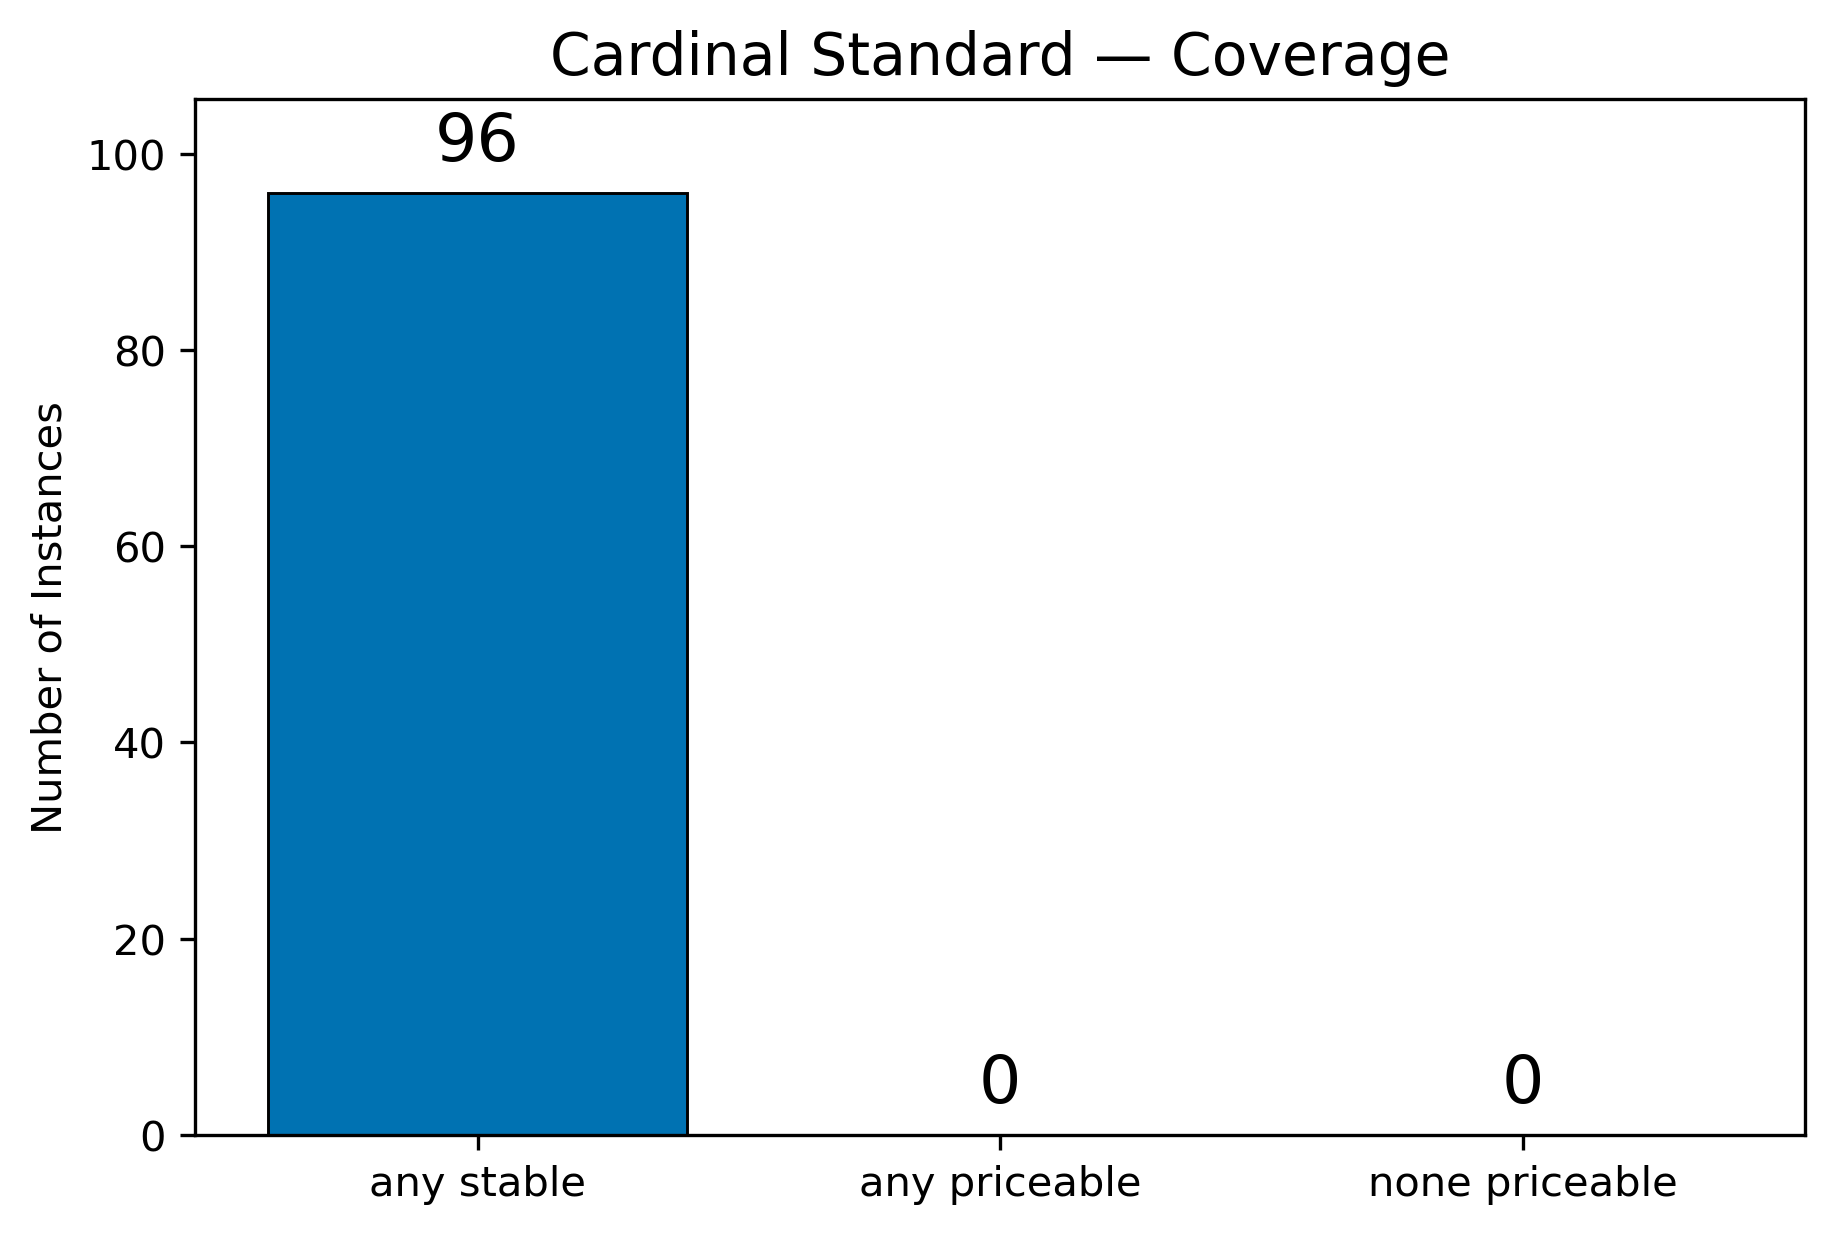
\includegraphics[width=0.7\textwidth]{figures/plots/cardinal-standard/cardinal_standard_coverage_non_exhaustive.png}
  \caption{Number of instances of elections for standard cardinal-based elections, for which any rule was able to return a stable priceable, or a priceable allocation.}
  \label{fig:myplot}
\end{figure}
\begin{figure}[H]         
  \centering              
  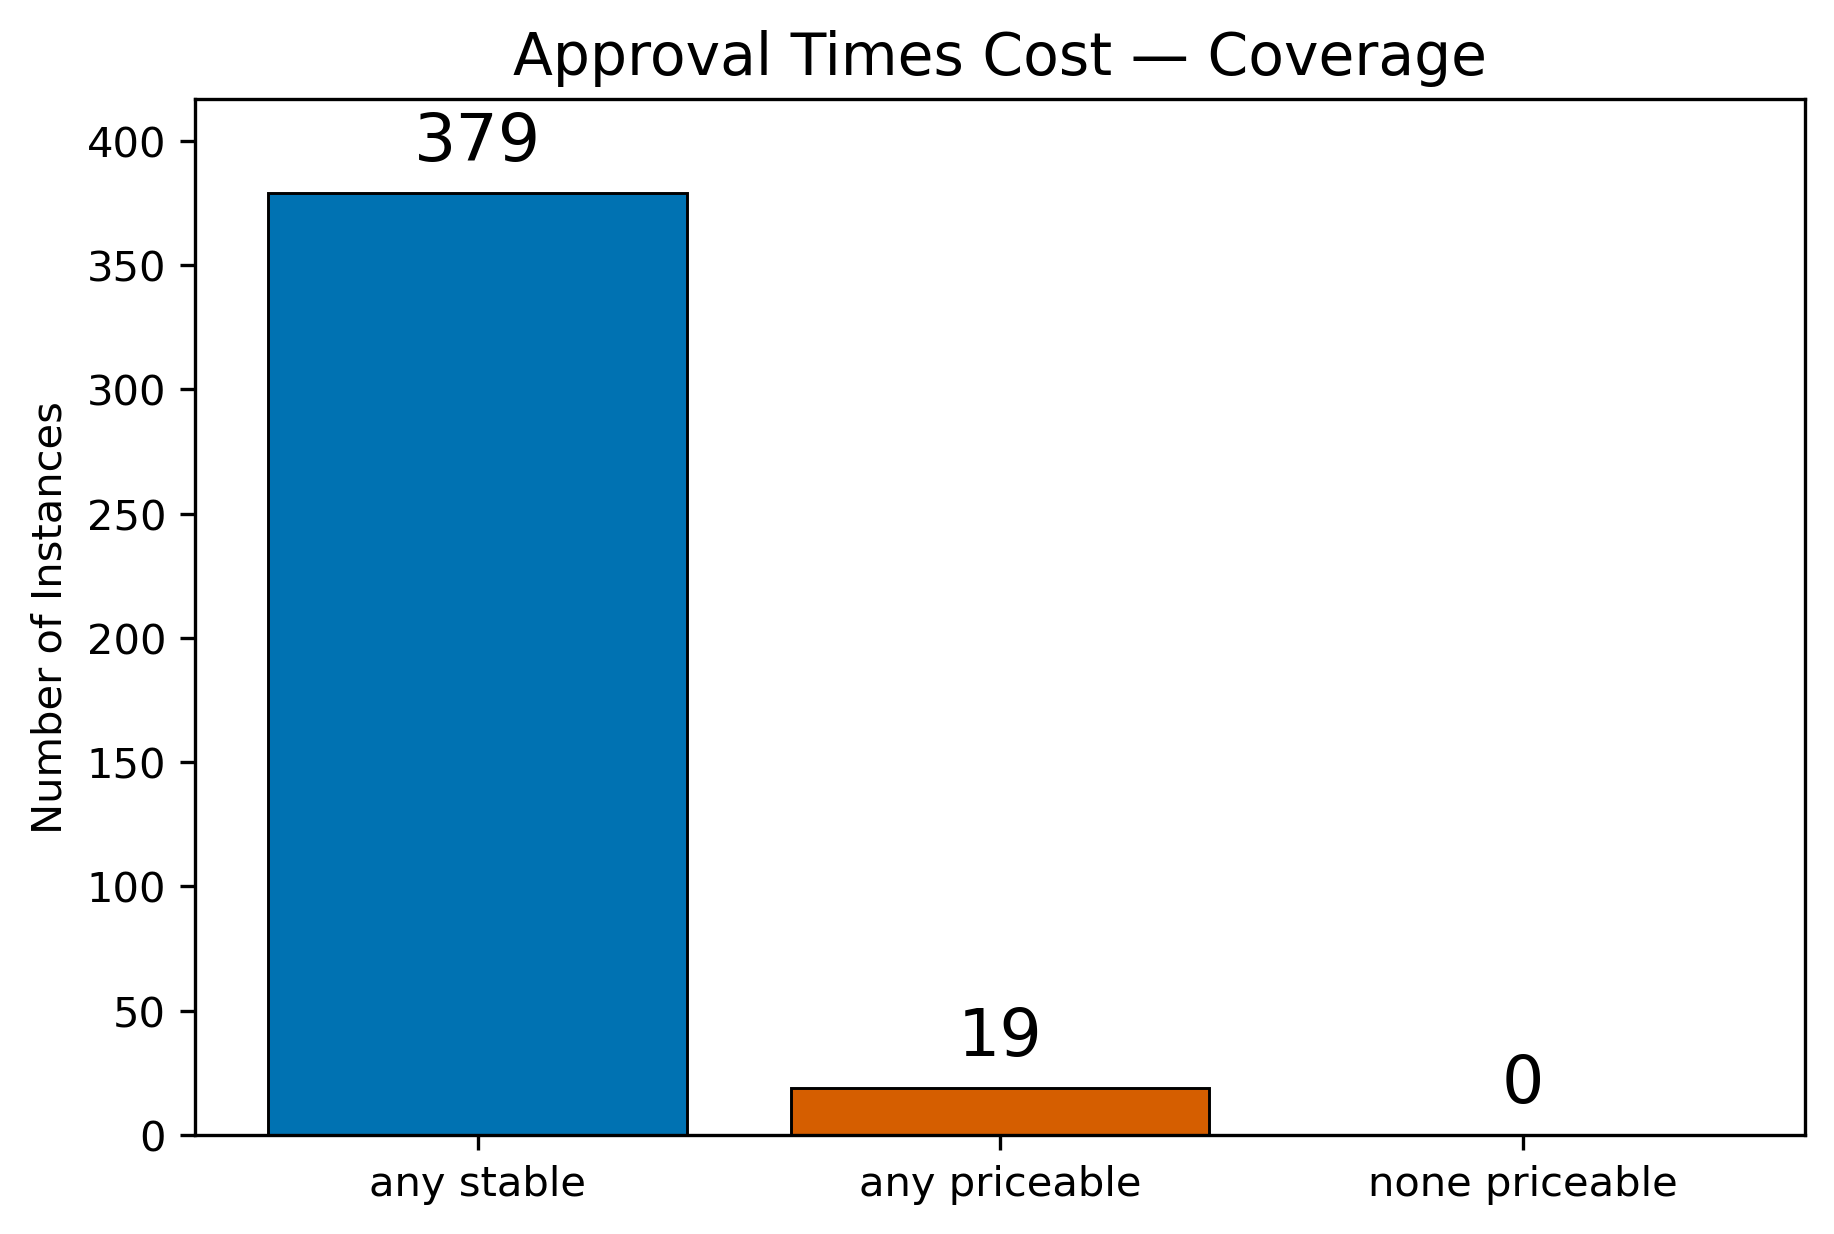
\includegraphics[width=0.7\textwidth]{figures/plots/approval-times-cost/approval_times_cost_coverage_non_exhaustive.png}
  \caption{Number of instances of elections for standard approval-based ballot instances multiplied by projects' costs, for which any rule was able to return a stable priceable, or a priceable allocation.}
  \label{fig:myplot}
\end{figure}
\begin{figure}[H]         
  \centering              
  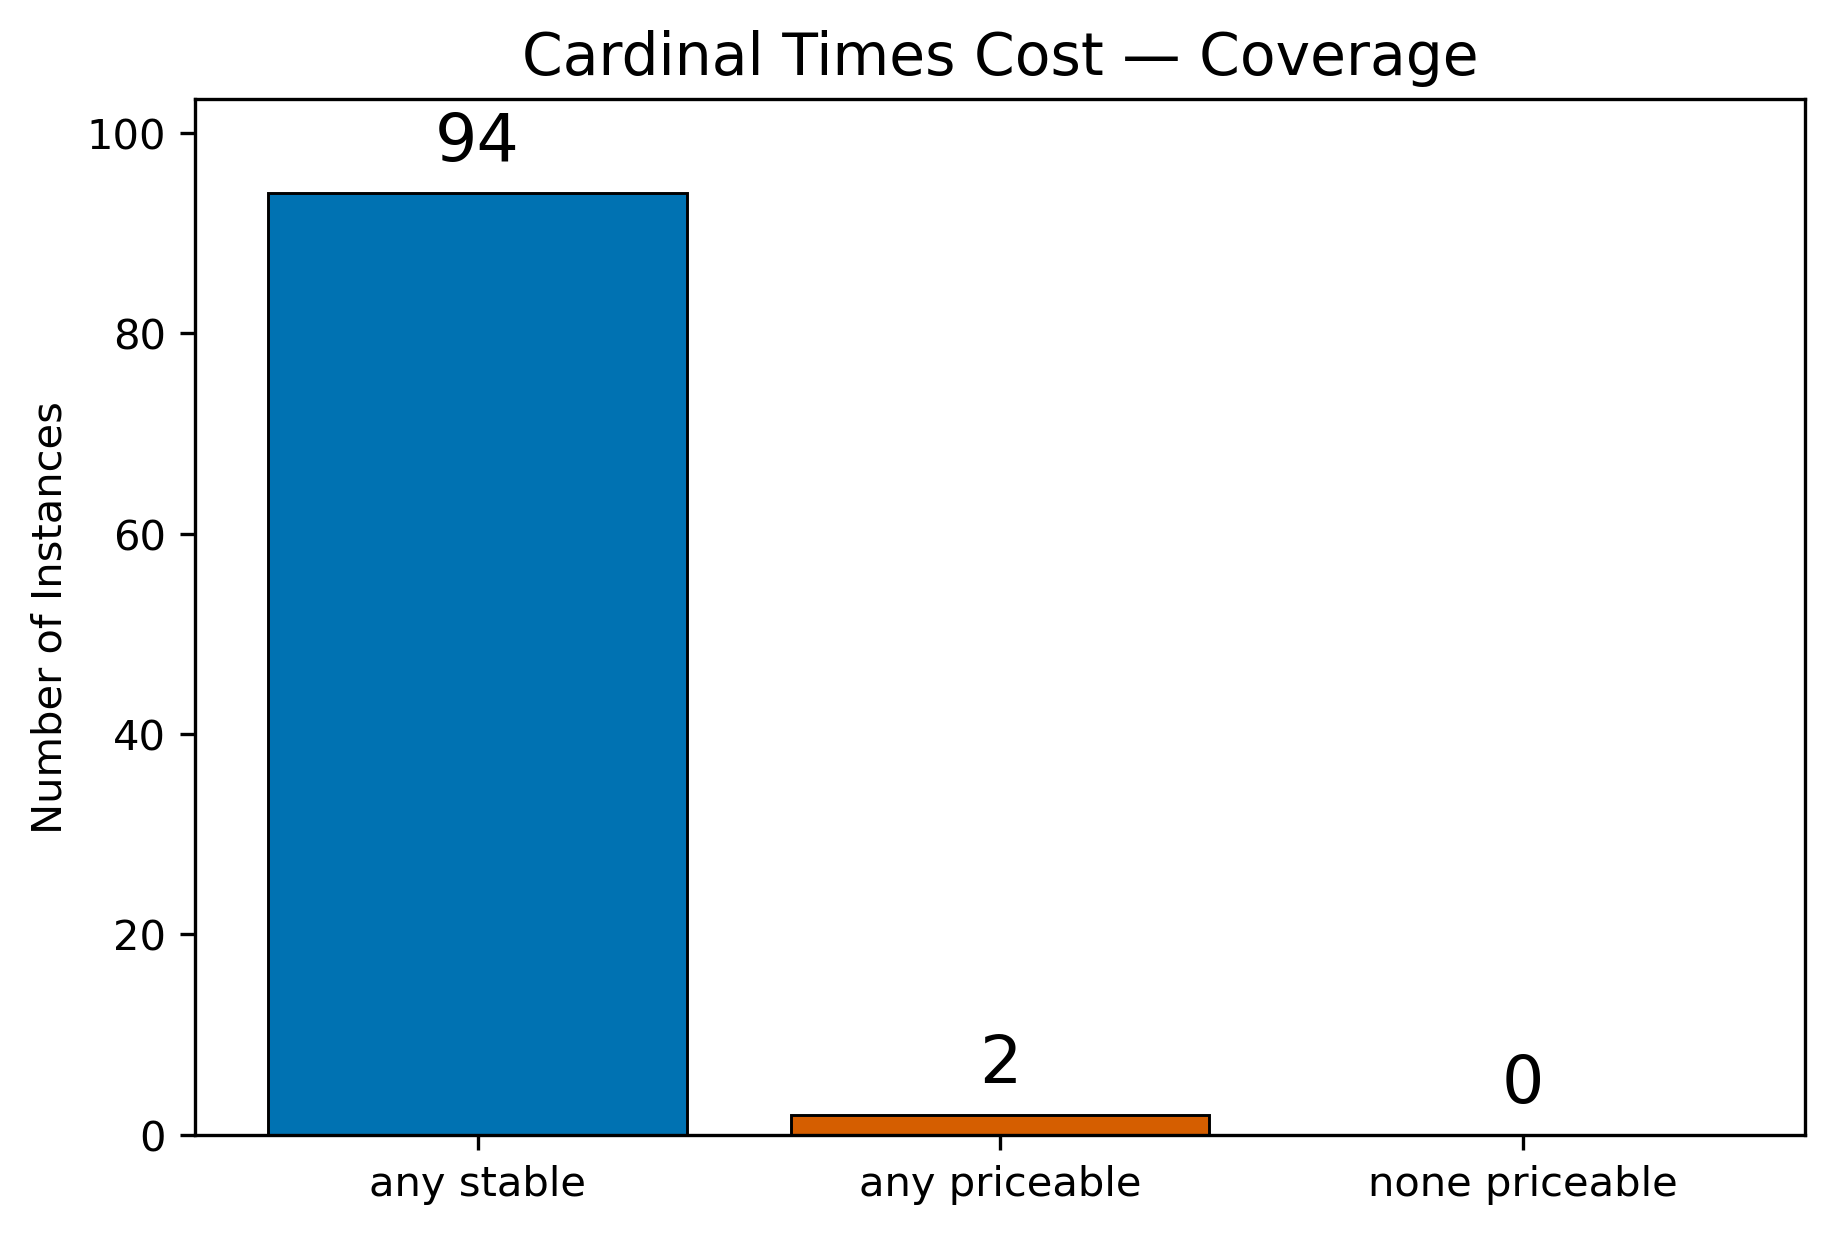
\includegraphics[width=0.7\textwidth]{figures/plots/cardinal-times-cost/cardinal_times_cost_coverage_non_exhaustive.png}
  \caption{Number of instances of elections for standard cardinal-based ballot instances multiplied by projects' costs, for which any rule was able to return a stable priceable, or a priceable allocation.}
  \label{fig:myplot}
\end{figure}
A priceable solution was always found. However --- when using cost satisfaction measure, we observe that a stable priceable solution was not always returned by any of the tested methods. This does not mean, that the methods behaved poorly, as such solutions might not always exist.
\begin{figure}[H]         
  \centering              
  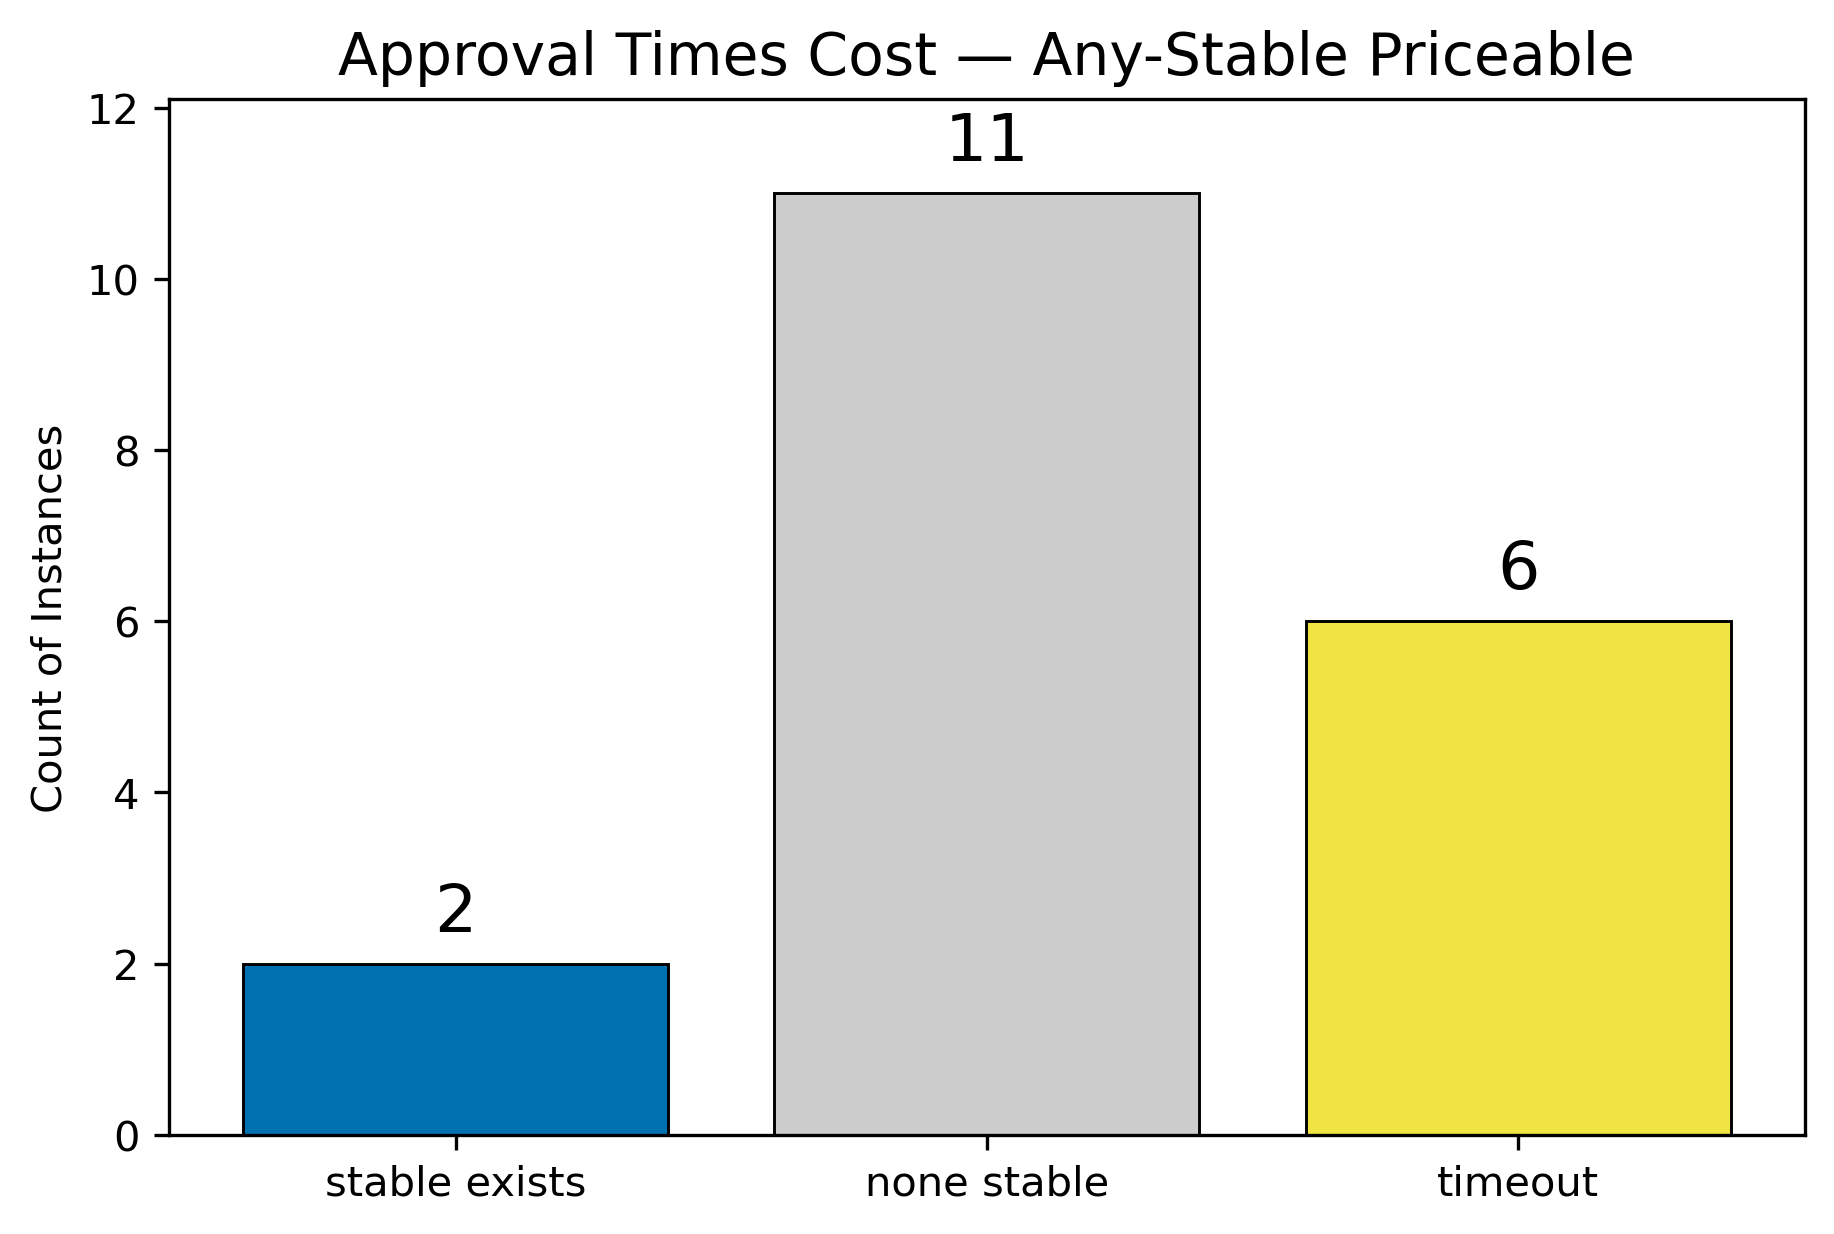
\includegraphics[width=0.7\textwidth]{figures/plots/approval-times-cost/approval_times_cost_any_stable_non-exhaustive.png}
  \caption{Number of instances of elections with approval ballots and cost satisfaction measure, for which no election rule returned a stable priceable allocation, where such a solution exists or does not.}
  \label{fig:myplot}
\end{figure}
\begin{figure}[H]         
  \centering              
  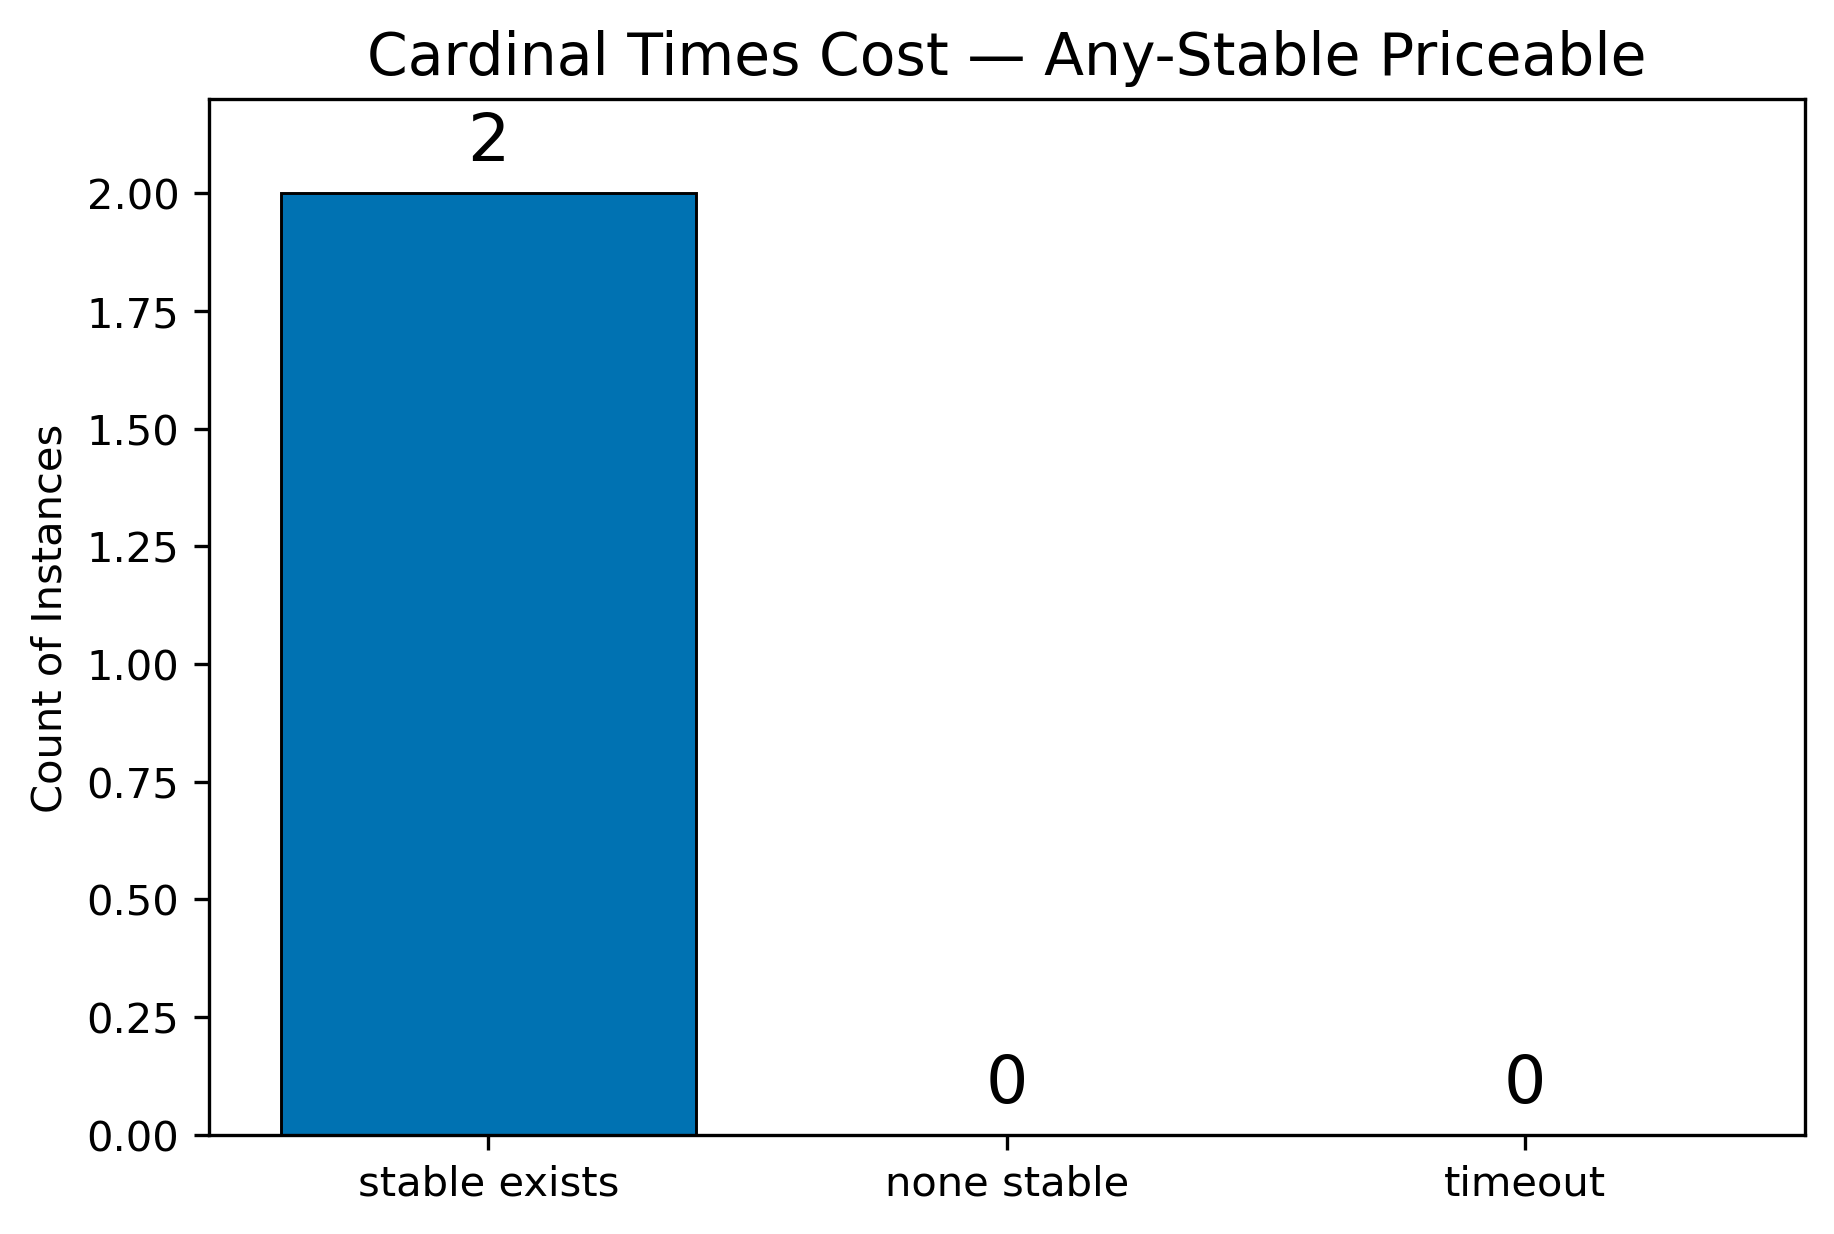
\includegraphics[width=0.7\textwidth]{figures/plots/cardinal-times-cost/cardinal_times_cost_any_stable_non-exhaustive.png}
  \caption{Number of instances of elections with cardinal ballots and cost satisfaction measure, for which no election rule returned a stable priceable allocation, where such a solution exists or does not.}
  \label{fig:myplot}
\end{figure}
In majority of cases, no stable priceable solution exists at all, meaning evaluated election rules did exceptionally well at finding existing stable priceable allocations. We also note a number of elections, when the \emph{priceable} function timed out within our time limit for the largest election instances. We accept this, as finding an allocation is a more difficult task than pure evaluation of a given result, and see this as area for further research with stronger computers and larger time limits.
\section{Exhaustive priceable and stable priceable outcomes}
As previously stated, it is highly beneficial for an election rule to return stable priceable, or at least, priceable outcomes. 

However, it is known that there exist election instances which do not have exhaustive priceable allocations. We say that an allocation is exhaustive if no unchosen project can be added to the allocation, without going over the total budget.
\begin{example}
Consider the following simple election with total budget $b:=3$, where choosing the only exhaustive allocation involves selecting a candidate with no supporters.
\begin{table}[H]
\centering
\begin{tabular}{lllccc}
\toprule
        & cost & $\#app$ & $v_1$ & $v_2$ & $v_3$\\
\midrule
\rowcolor{orange!10}
$c_1$& 1 & 0 & & &   \\
\rowcolor{orange!10}
$c_2$& 1 & 1 &  \app &  &        \\
\rowcolor{orange!10}
$c_3$& 1 & 2 &   & \app  & \app           \\
\bottomrule
\end{tabular}
\end{table}
It is clear that only choosing all candidates is exhaustive. However, that would mean that candidate $c_1$ also collects the total payment of $cost(c_1)=1$, which is against the notion that voters are only allowed to contribute funds towards candidates that they approve of.
\end{example}
It is usually sensible, to try to obtain exhaustive results. Intuitively, in a participatory budgeting setting, no voters would be against adding another project to the outcome, since they could either benefit from it or simply be indifferent to it in terms of their satisfaction. There are no obvious advantages to choosing non-exhaustive election rules in a a PB setting. 

While the Utilitarian greedy method is exhaustive by default, the Method of Equal Shares is not. This property of MES is meant to be fixed by its $2$ variations, including voter budget increment and greedy fill. BOS is also not exhaustive.

In this section, we look at the results obtained from all previously mentioned election rules and check, in how many instances they returned an exhaustive priceable or stable priceable outcome and which rule performed best.
\begin{figure}[H]         
  \centering              
  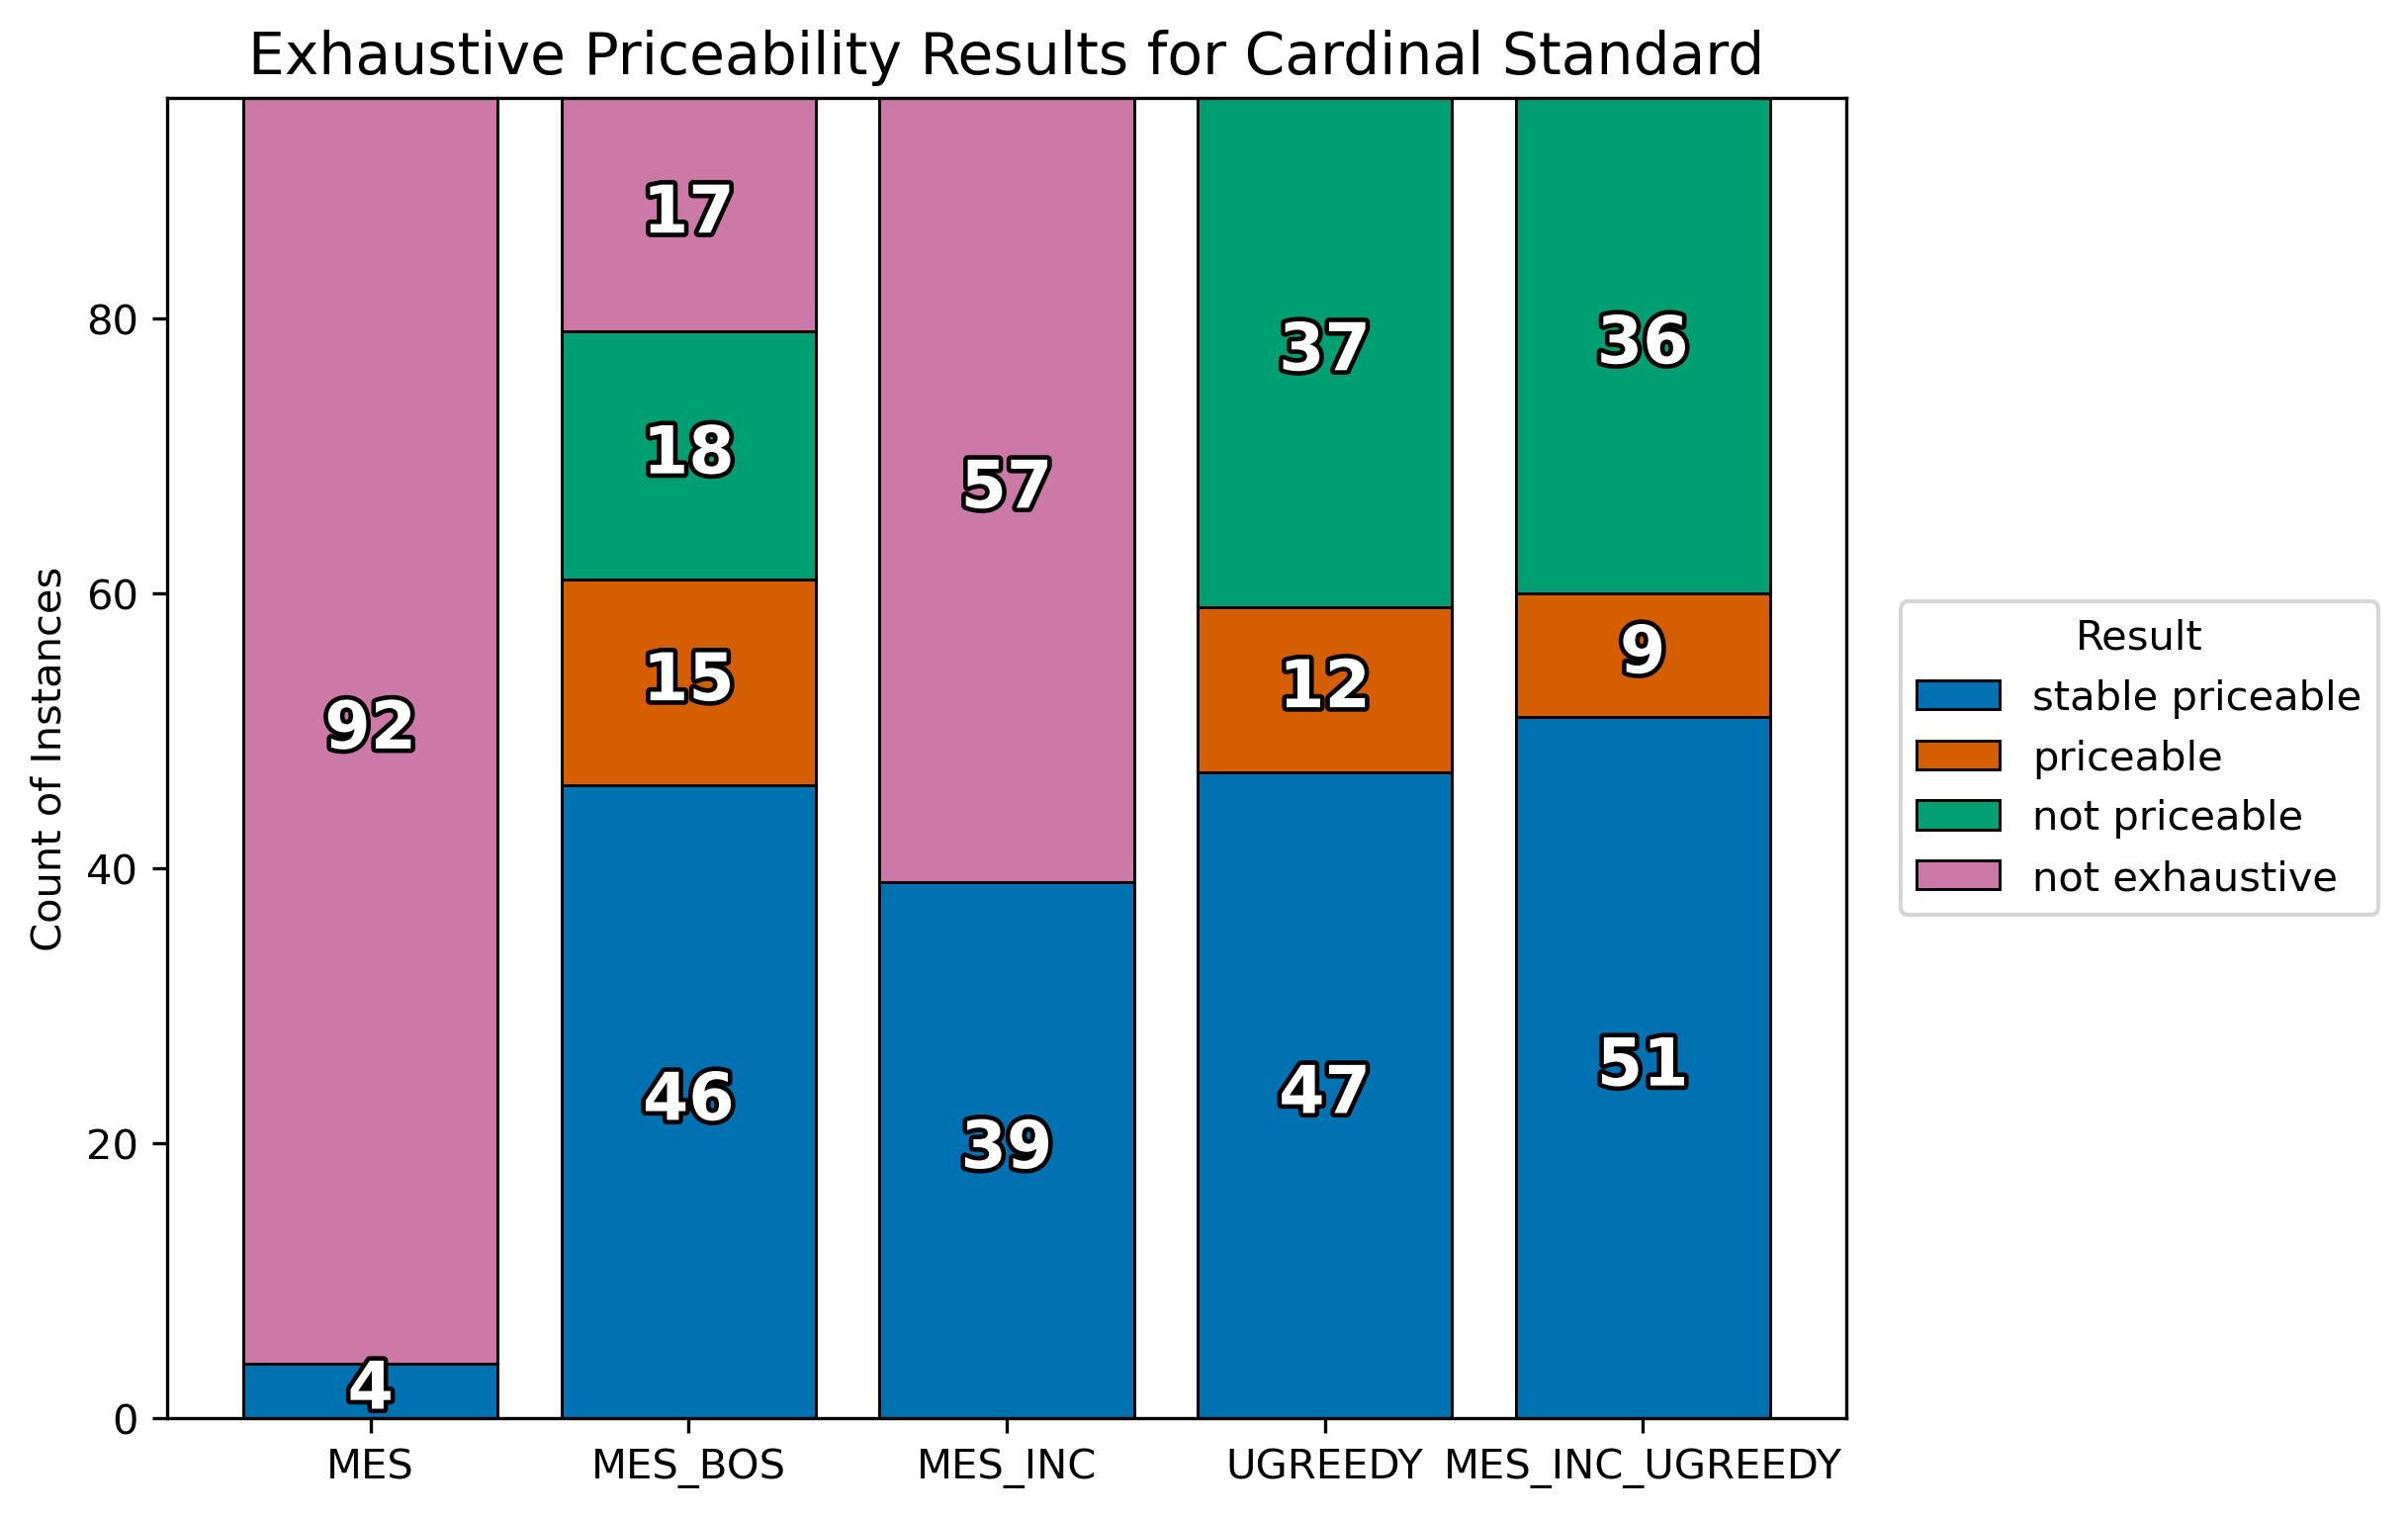
\includegraphics[width=0.7\textwidth]{figures/plots/cardinal-standard/cardinal_standard_exh_priceability.png}
  \caption{Exhaustive stable priceable and priceable allocations returned by selected election rules for unmodified cardinal-based elections.}
  \label{fig:myplot}
\end{figure}
\begin{figure}[H]         
  \centering              
  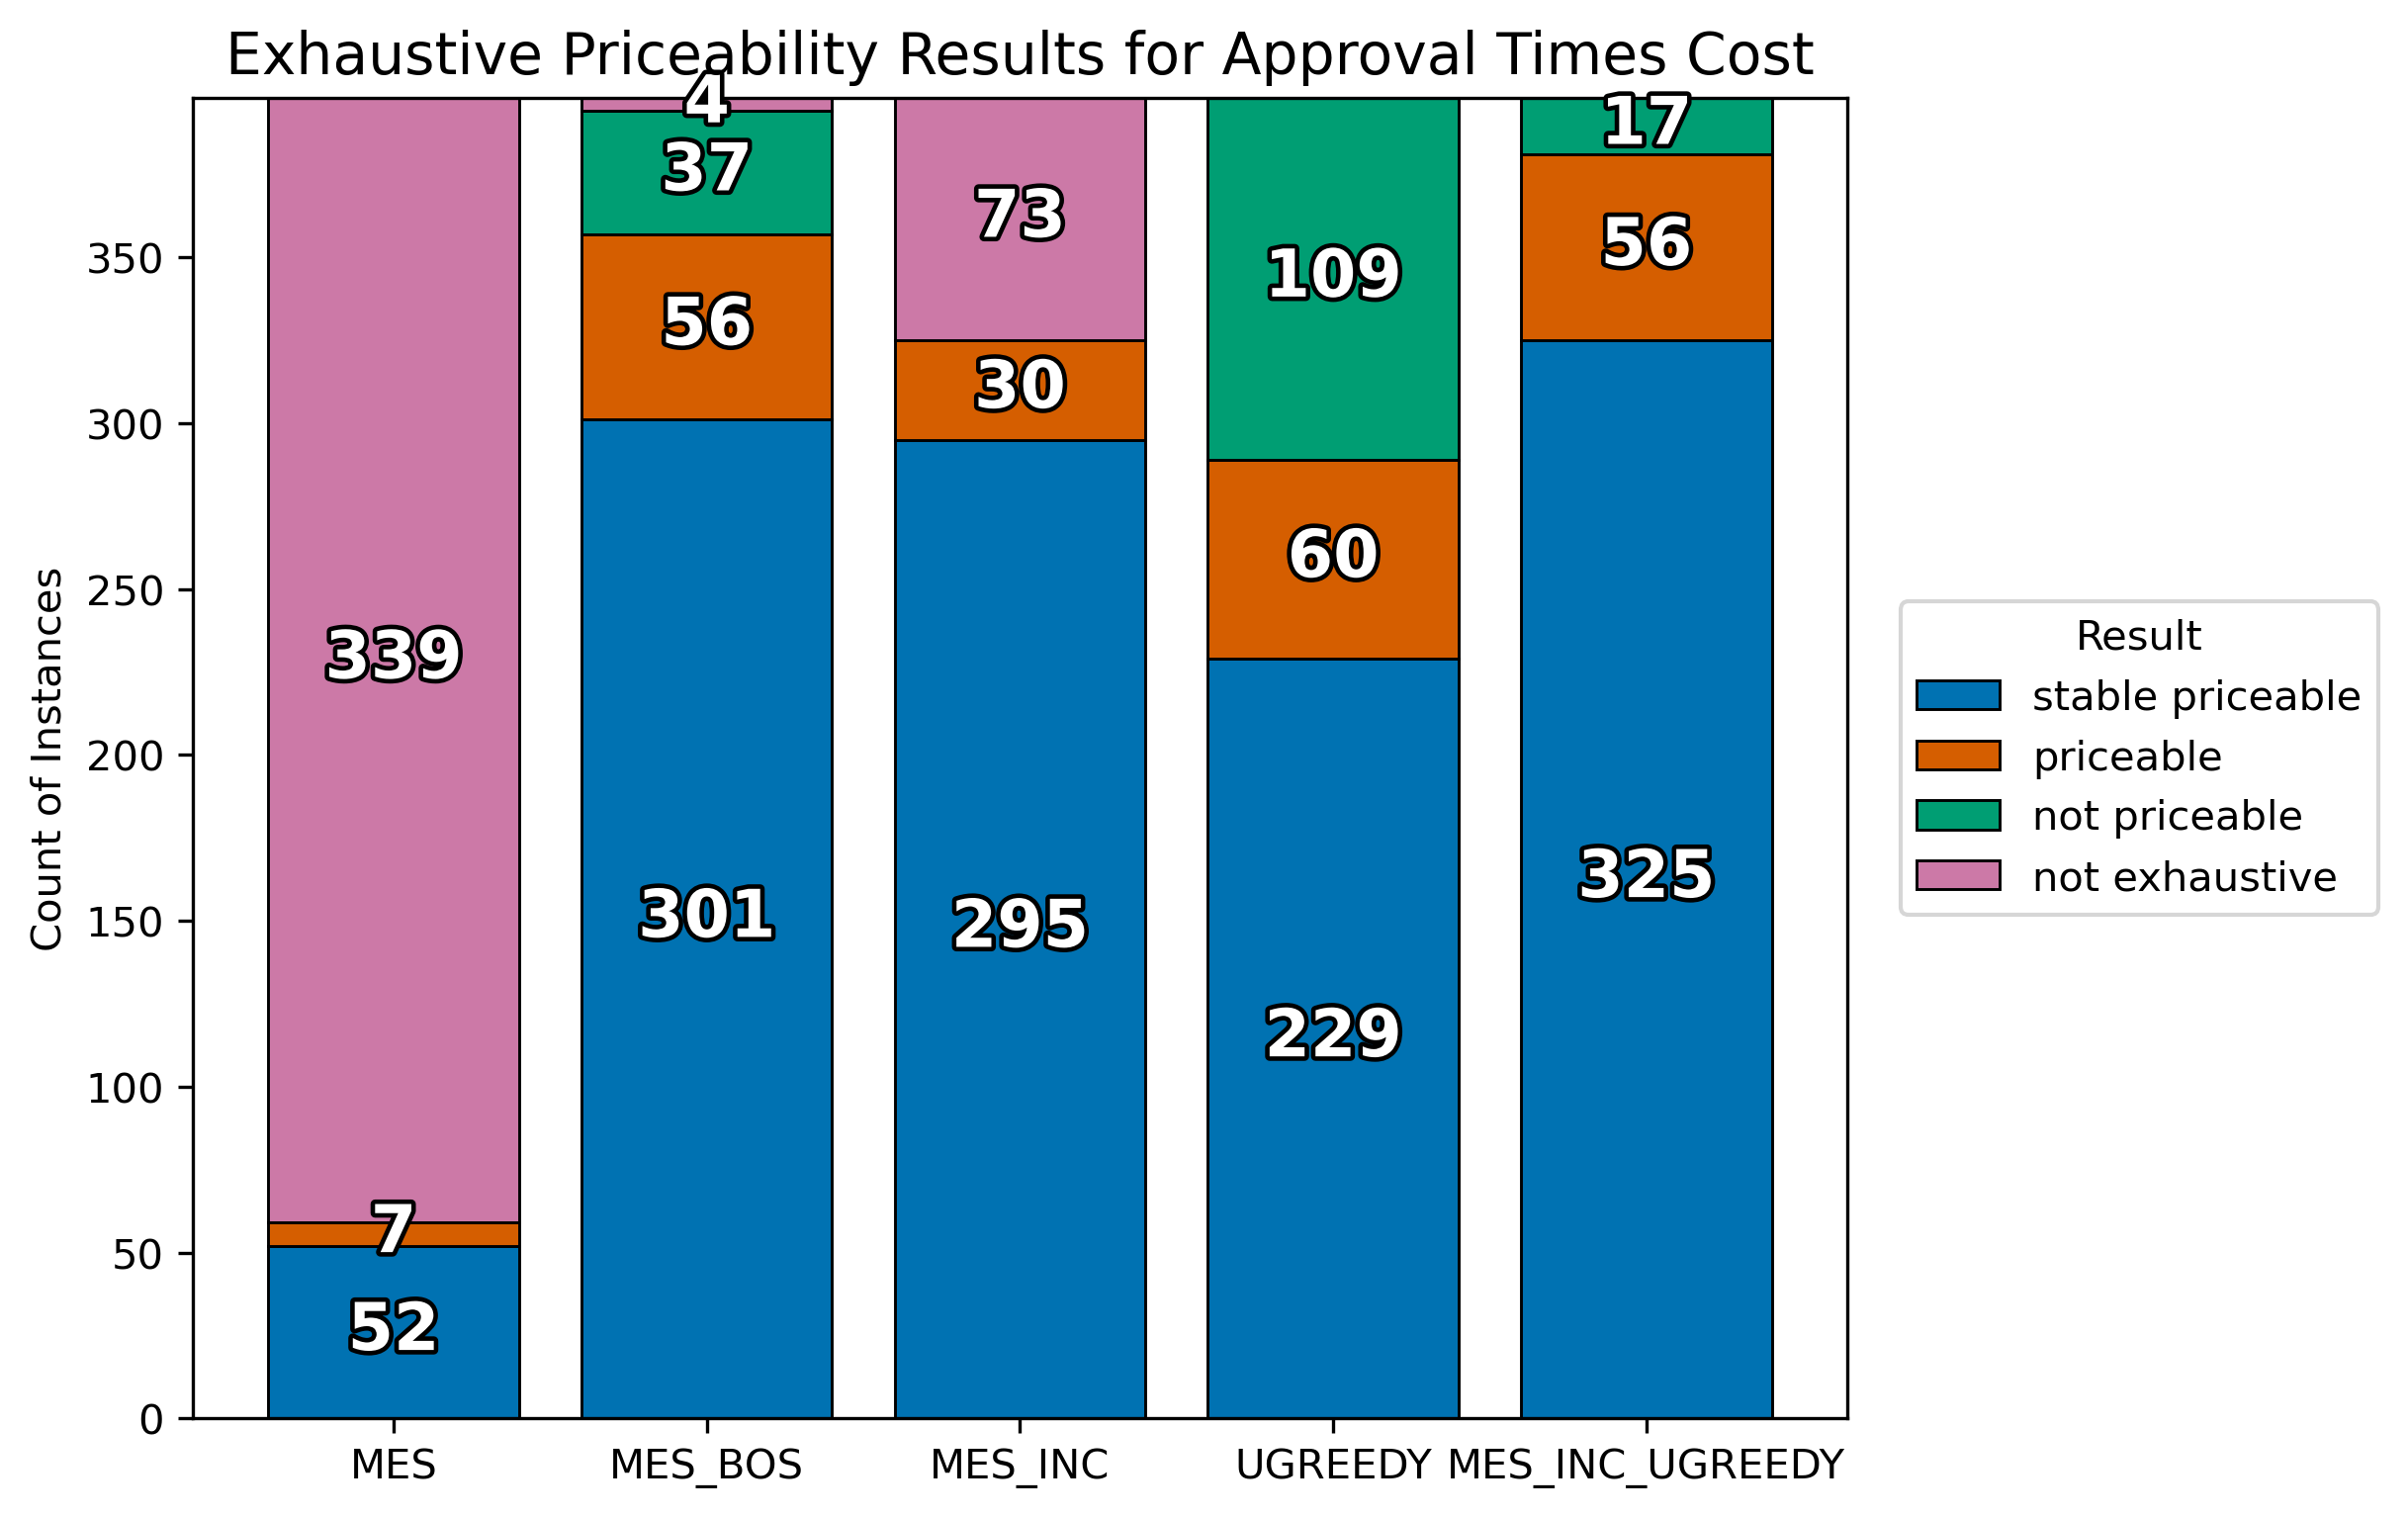
\includegraphics[width=0.7\textwidth]{figures/plots/approval-times-cost/approval_times_cost_exh_priceability.png}
  \caption{Exhaustive stable priceable and priceable allocations returned by selected election rules for approval-based elections with utilities multiplied by projects' costs.}
  \label{fig:myplot}
\end{figure}
\begin{figure}[H]         
  \centering              
  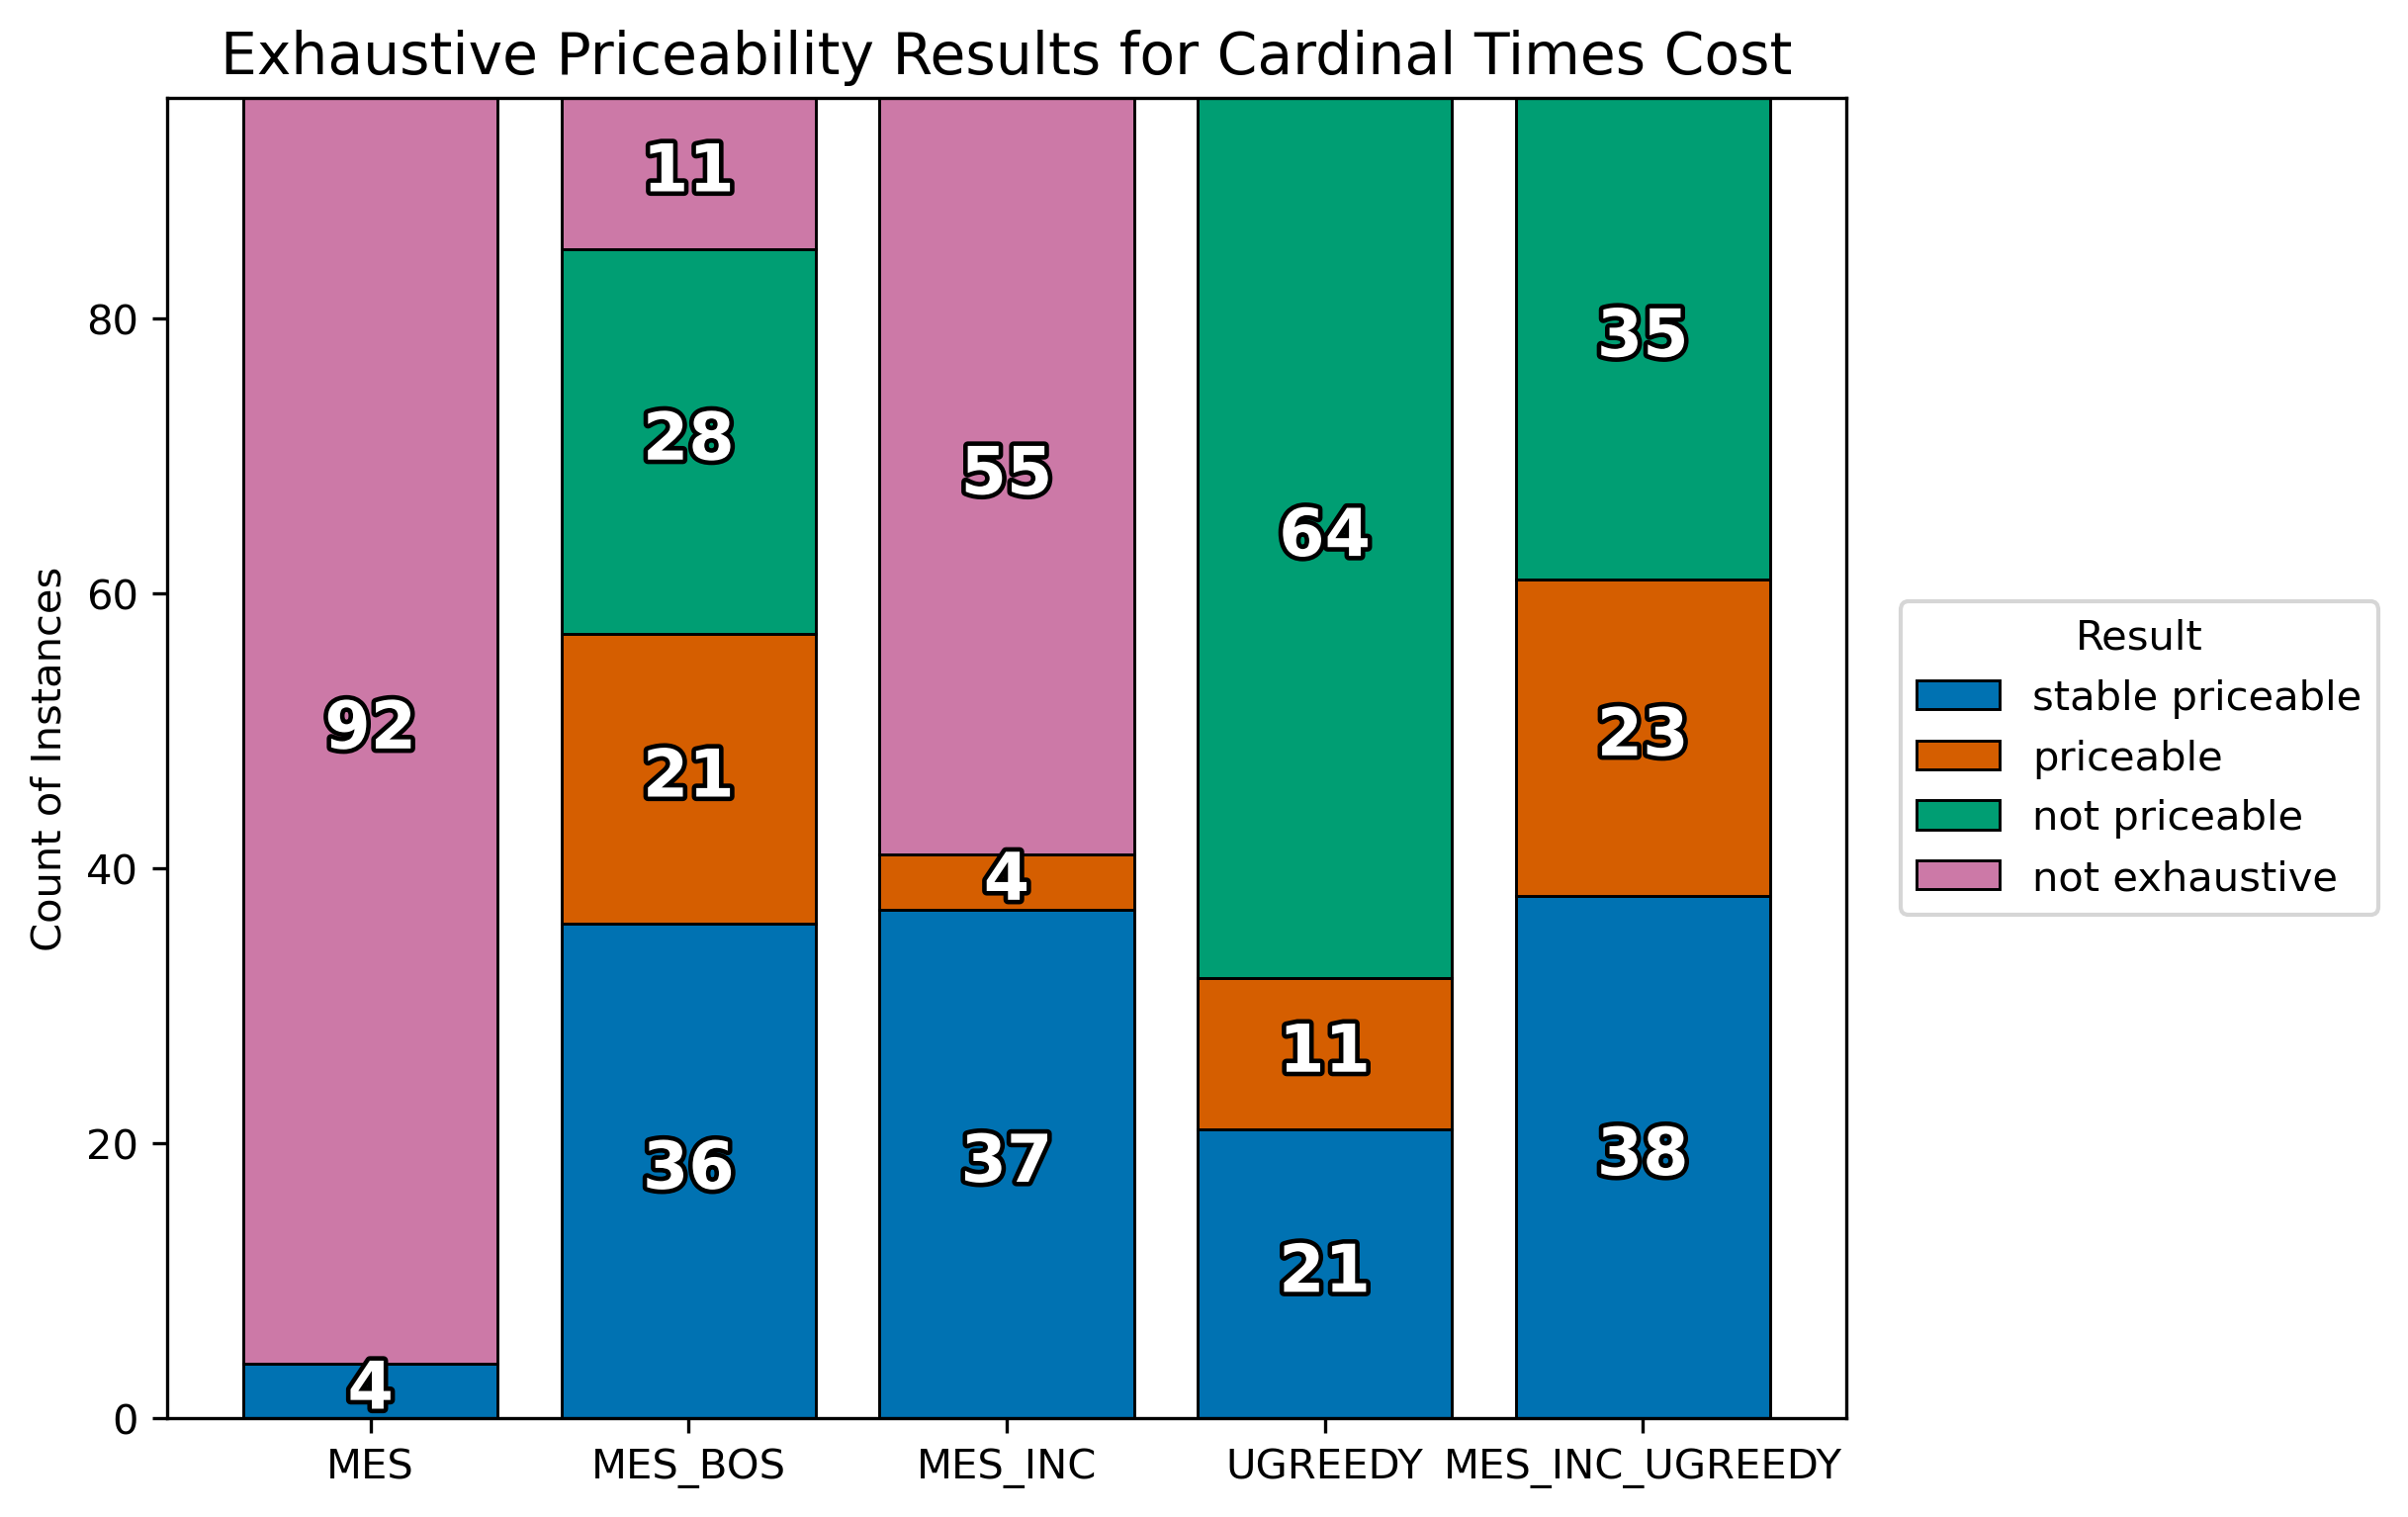
\includegraphics[width=0.7\textwidth]{figures/plots/cardinal-times-cost/cardinal_times_cost_exh_priceability.png}
  \caption{Exhaustive stable priceable and priceable allocations returned by selected election rules for approval-based elections with utilities multiplied by projects' costs.}
  \label{fig:myplot}
\end{figure}
As classic MES rarely returns exhaustive allocations at all, it almost never returns stable priceable exhaustive allocations, and it can be considered useless in this setting. However, when running the version with voter budget increment, its efficiency jumps to almost $74\%$ for approval elections with cost utilities and over $38\%$ for cardinal elections with cost utilities. Though BOS is not a variation meant to simply fix exhaustiveness, we observe significant improvements over classic MES. Utilitarian greedy scores just as well as with original constraints, and the same applies for MES with UGreedy fill. What stands out is that for elections originally in the cardinal setting, all methods do significantly worse compared to approval-based, though it was not visible without the exhaustive clause. It is either a sign of cost utilities being less proportional on their own, or that evaluated methods' approach does not efficiently grasp the concept of this kind of proportionality measurement.

So far, we have compared each rule’s ability to return stable priceable allocations and exhaustive stable priceable allocations. One natural question remains: of the allocations that are stable‐priceable when we do \emph{not} insist on exhaustiveness, how many remain stable‐priceable with the exhaustive clause? The following three pie-charts show, for each profile type and each rule, the fraction of previously stable‐priceable outcomes that still survive the exhaustive check (blue) versus those that do not (pink).
\begin{figure}[H]         
  \centering              
  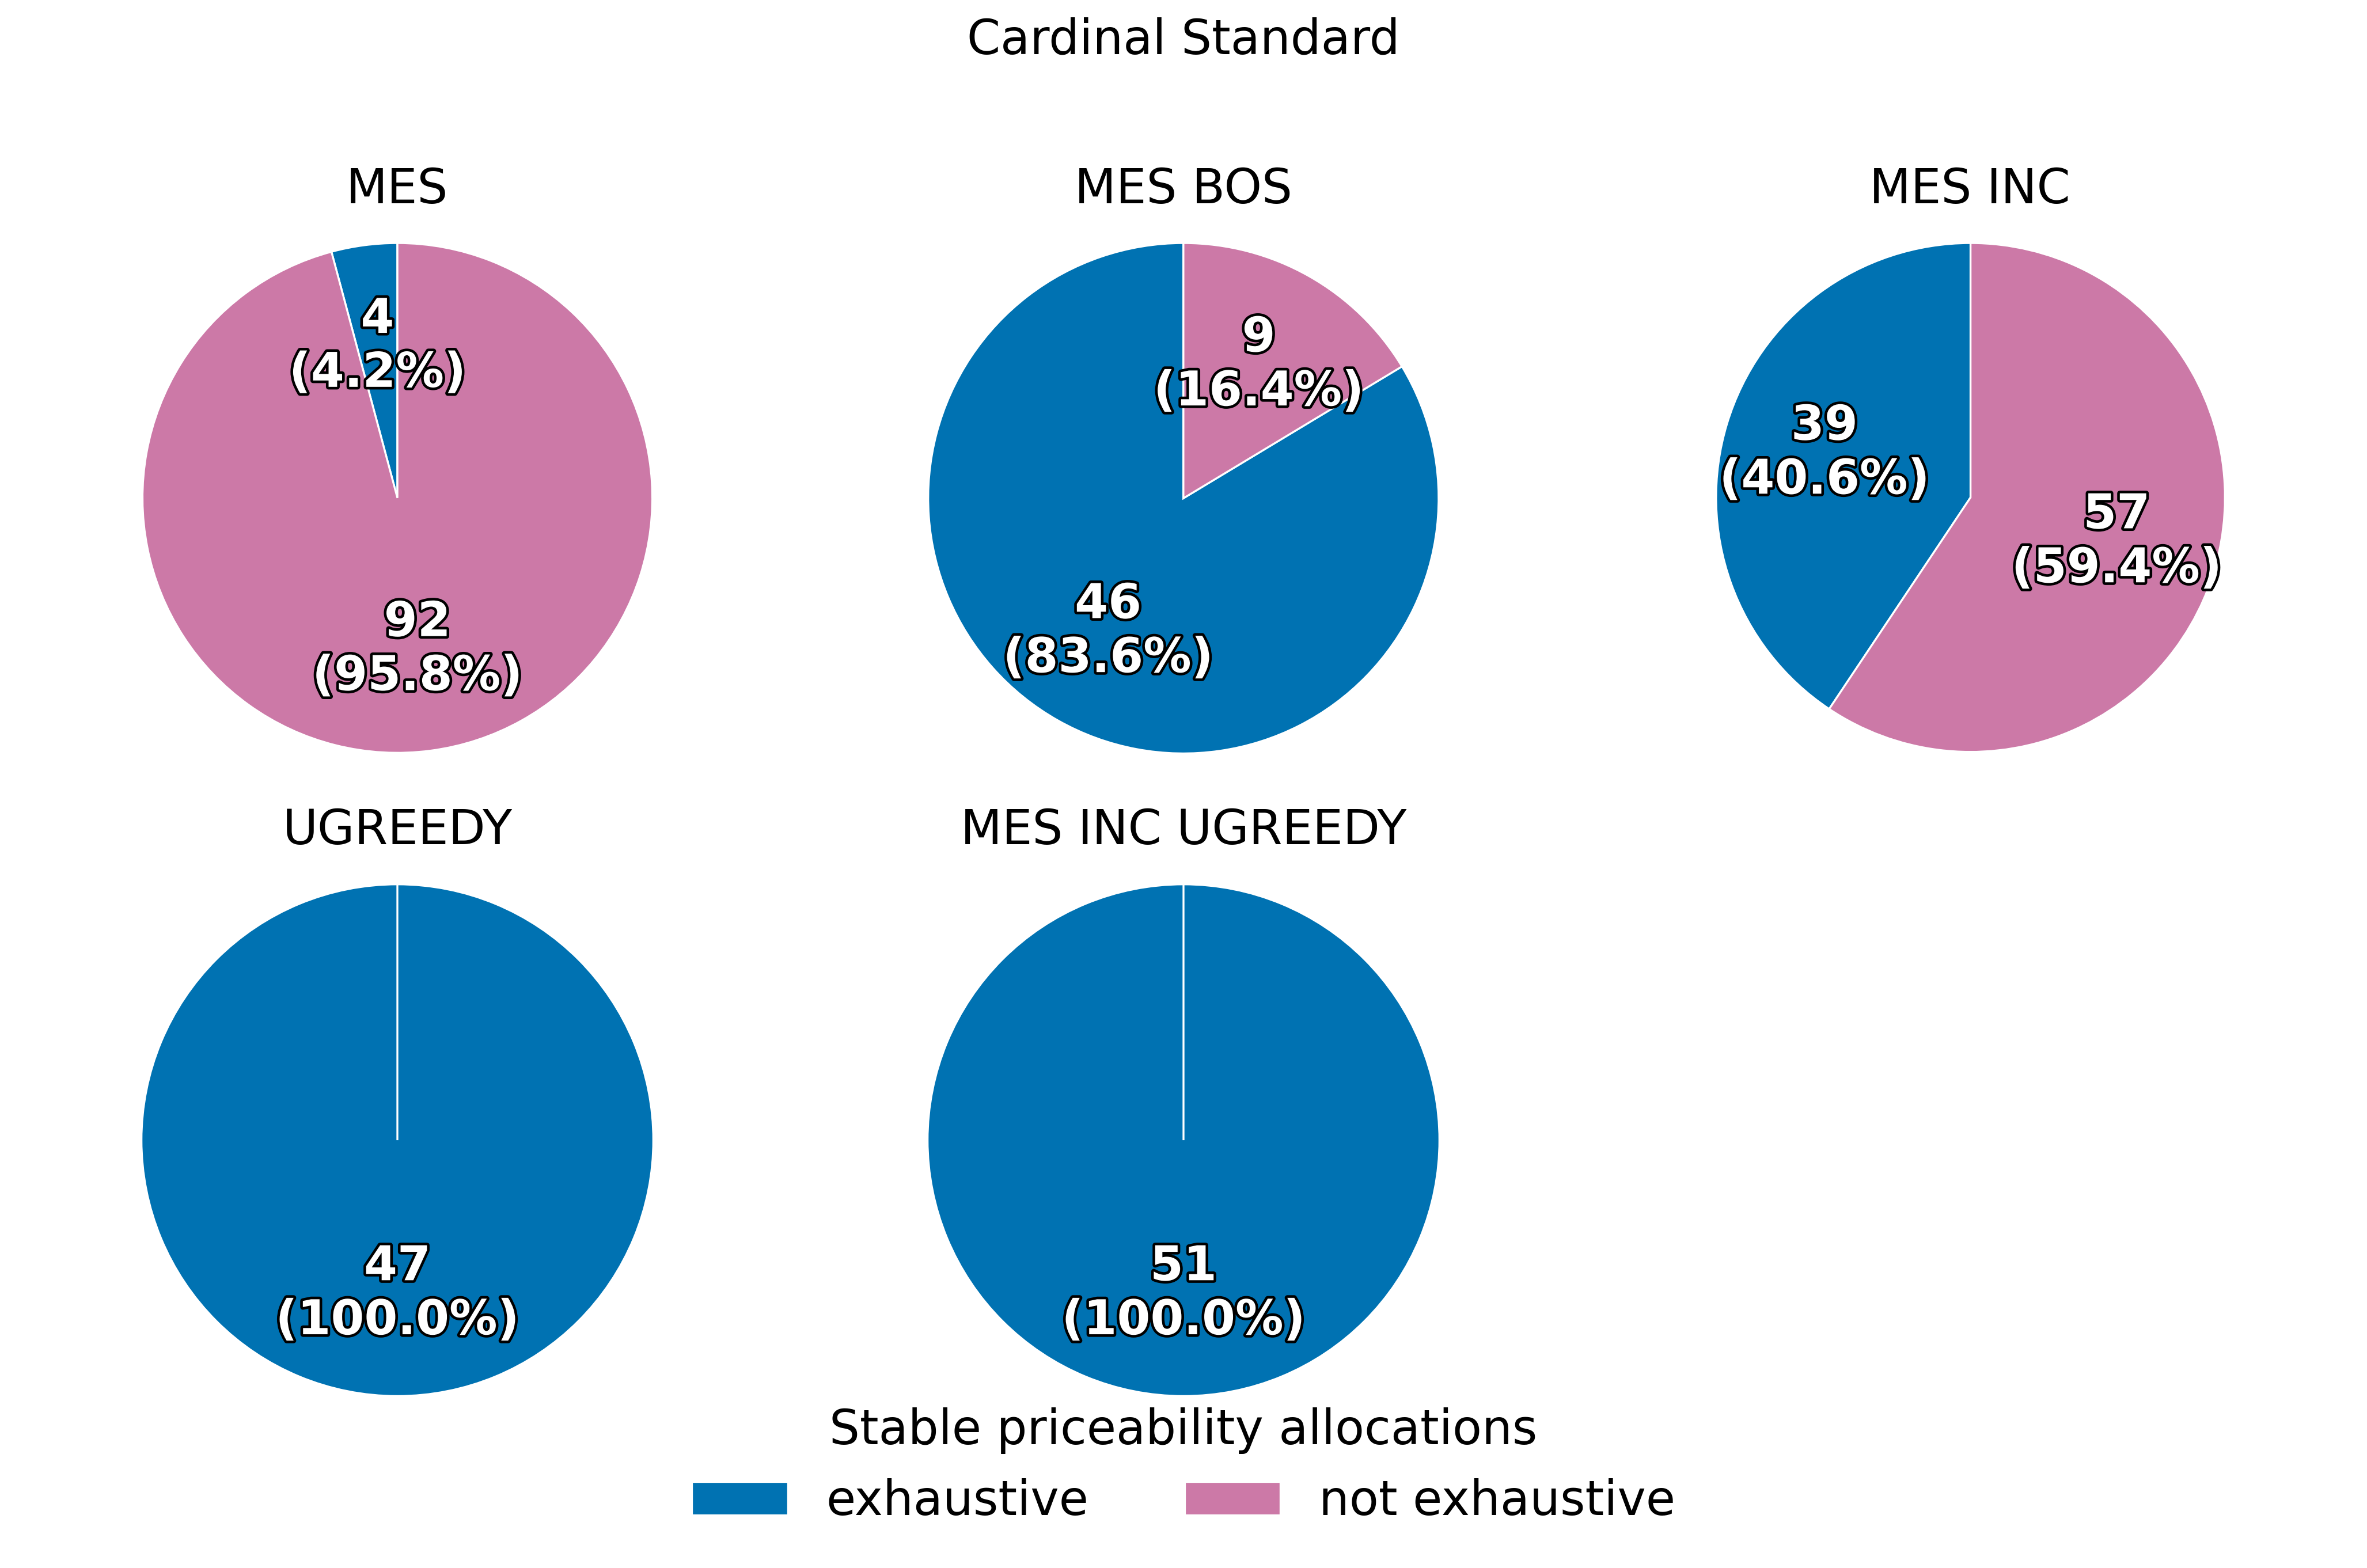
\includegraphics[width=0.7\textwidth]{figures/plots/cardinal-standard/cardinal_standard_stability_pies.png}
  \caption{Percentage of stable priceable allocations being exhaustive for cardinal-based ballots.}
  \label{fig:myplot}
\end{figure}

\begin{figure}[H]         
  \centering              
  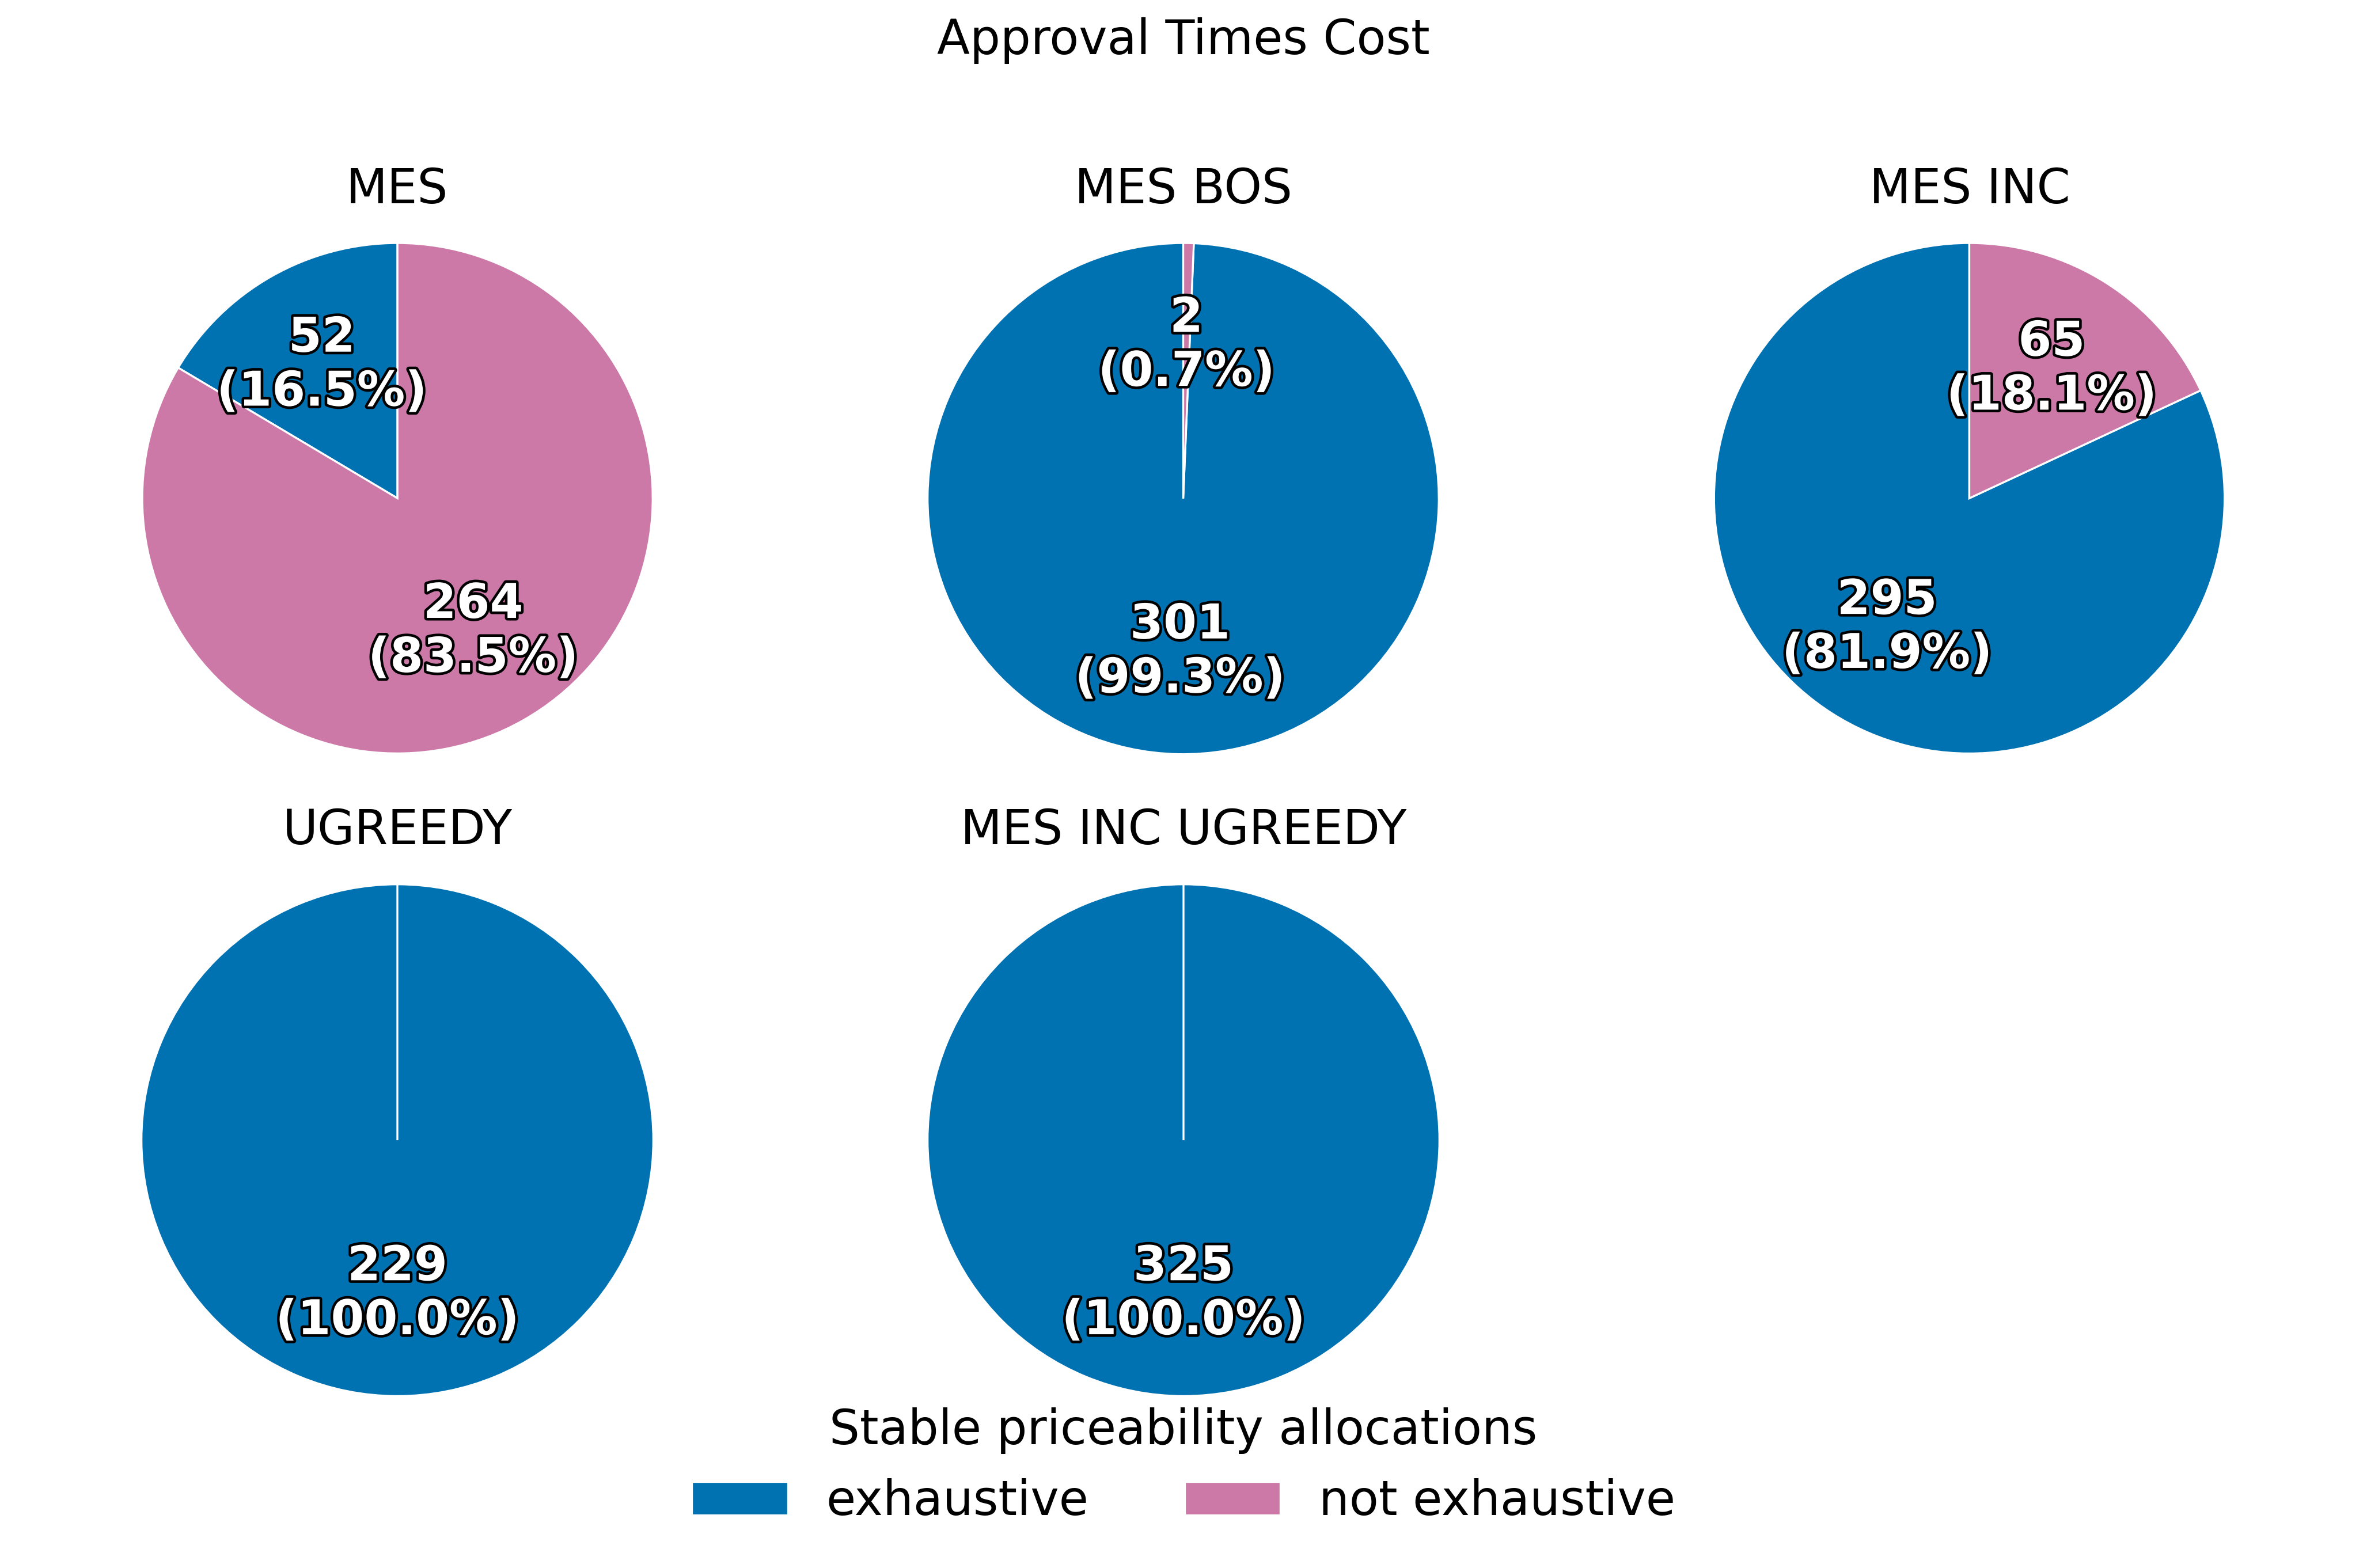
\includegraphics[width=0.7\textwidth]{figures/plots/approval-times-cost/approval_times_cost_stability_pies.png}
  \caption{Percentage of stable priceable allocations being exhaustive for approval-based ballots adjusted to cost utility.}
  \label{fig:myplot}
\end{figure}

\begin{figure}[H]         
  \centering              
  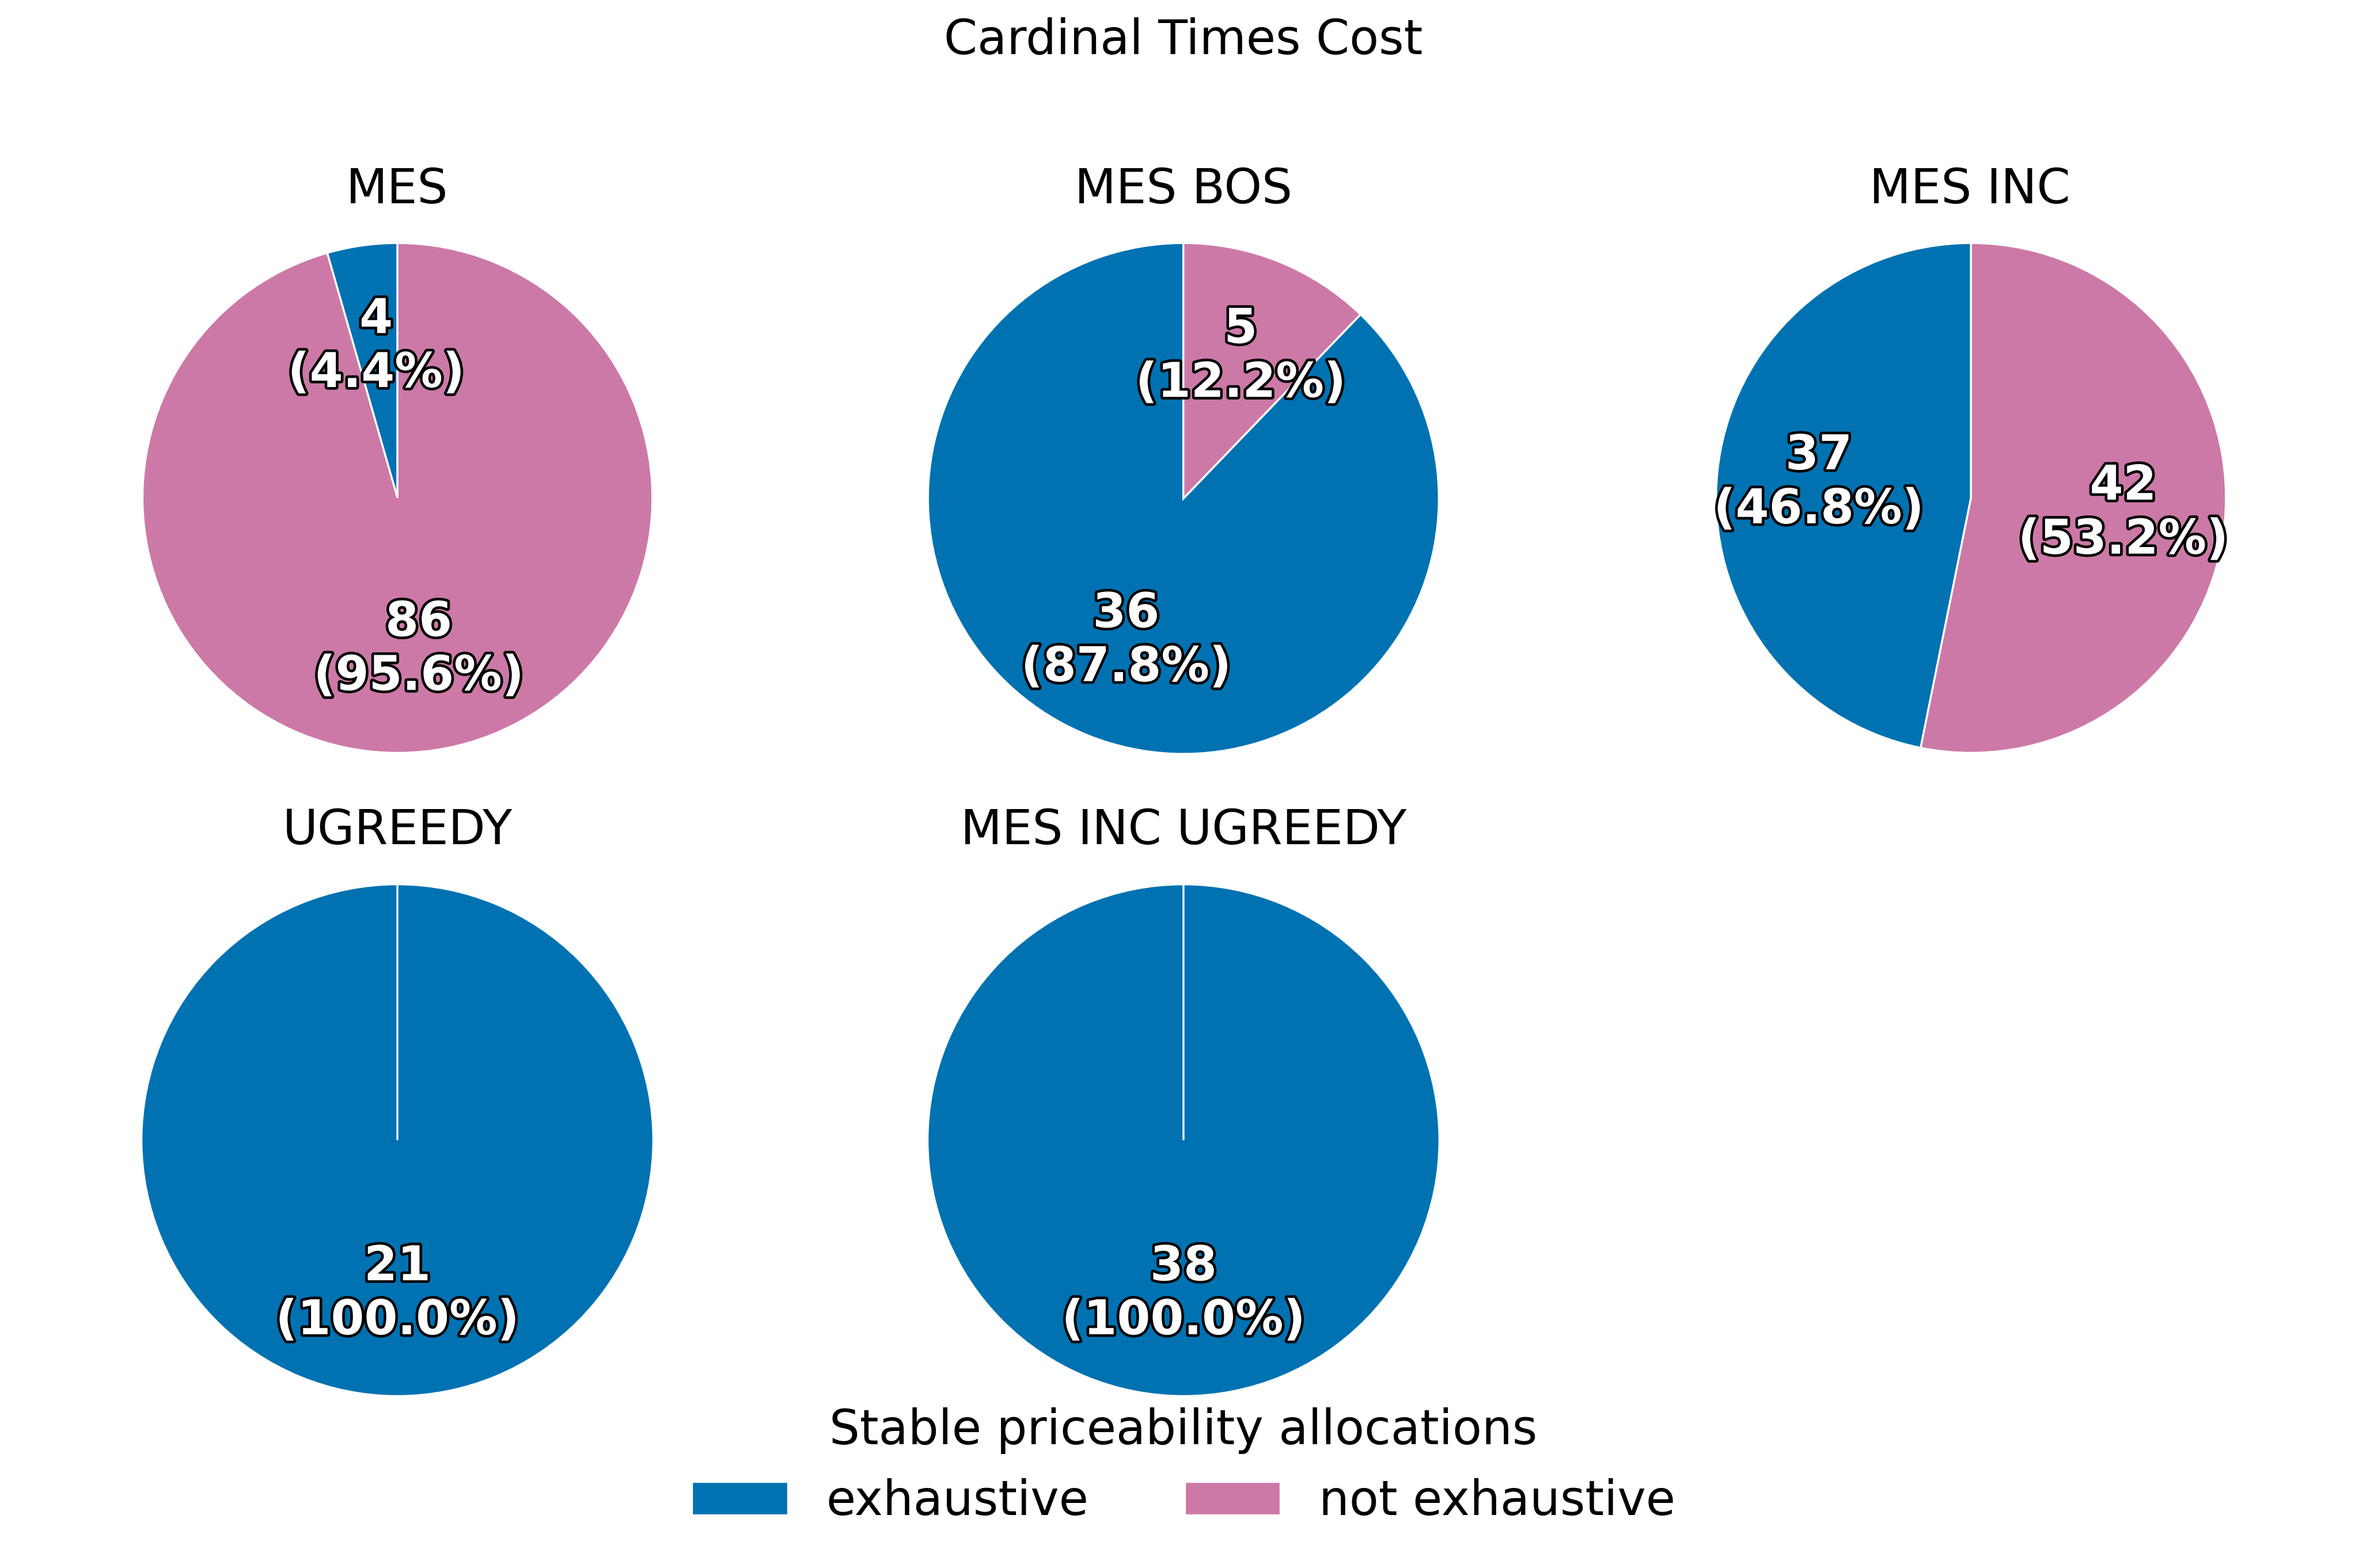
\includegraphics[width=0.7\textwidth]{figures/plots/cardinal-times-cost/cardinal_times_cost_stability_pies.png}
  \caption{Percentage of stable priceable allocations being exhaustive for cardinal-based ballots adjusted to cost utility.}
  \label{fig:myplot}
\end{figure}


Next, we look at each kind of election and check if any of the election rules used in empirical evaluation is able to find a stable-priceable or a priceable solution.

\begin{figure}[H]         
  \centering              
  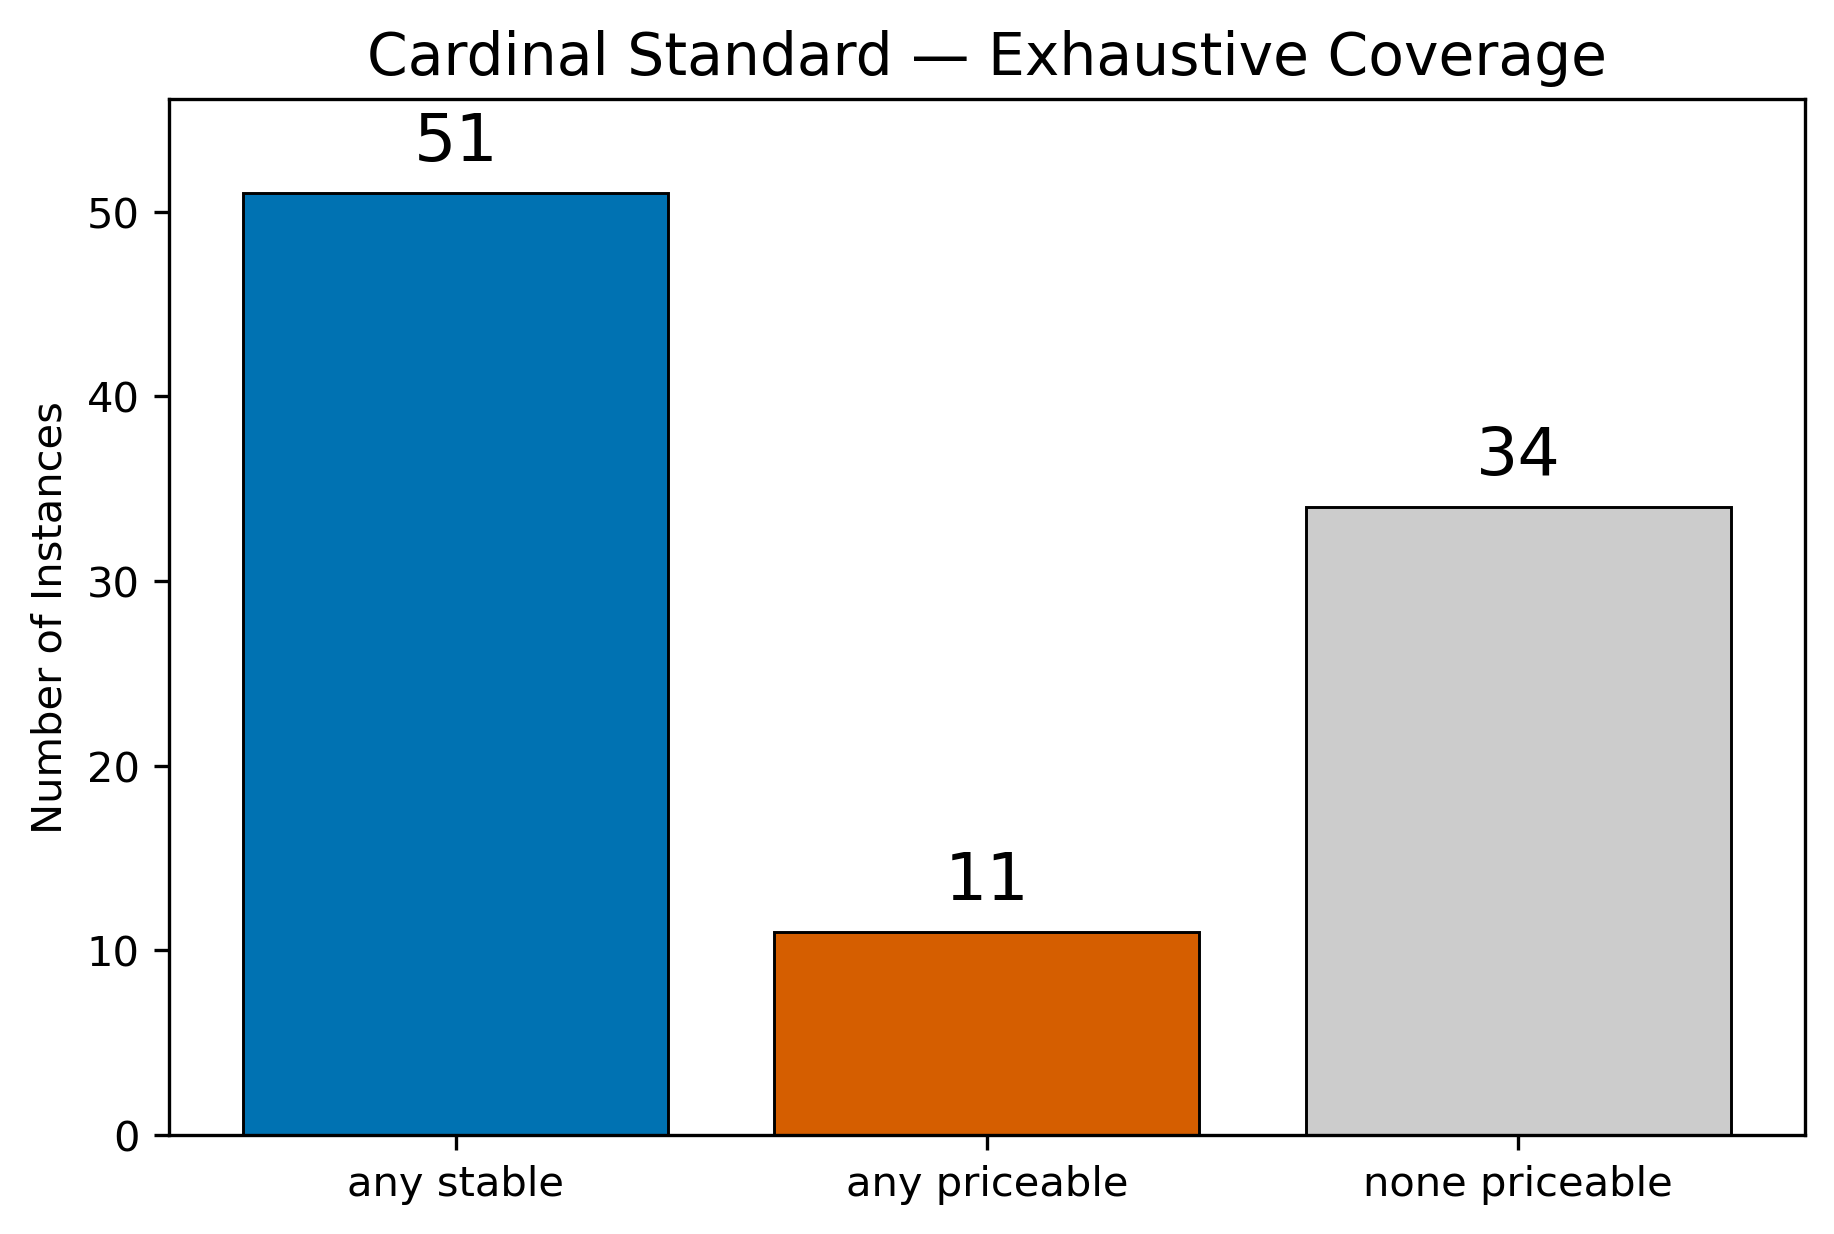
\includegraphics[width=0.7\textwidth]{figures/plots/cardinal-standard/cardinal_standard_coverage_exhaustive.png}
  \caption{Number of instances of standard cardinal-based elections, where at least one method return an exhaustive stable priceable or priceable allocation.}
  \label{fig:myplot}
\end{figure}
\begin{figure}[H]         
  \centering              
  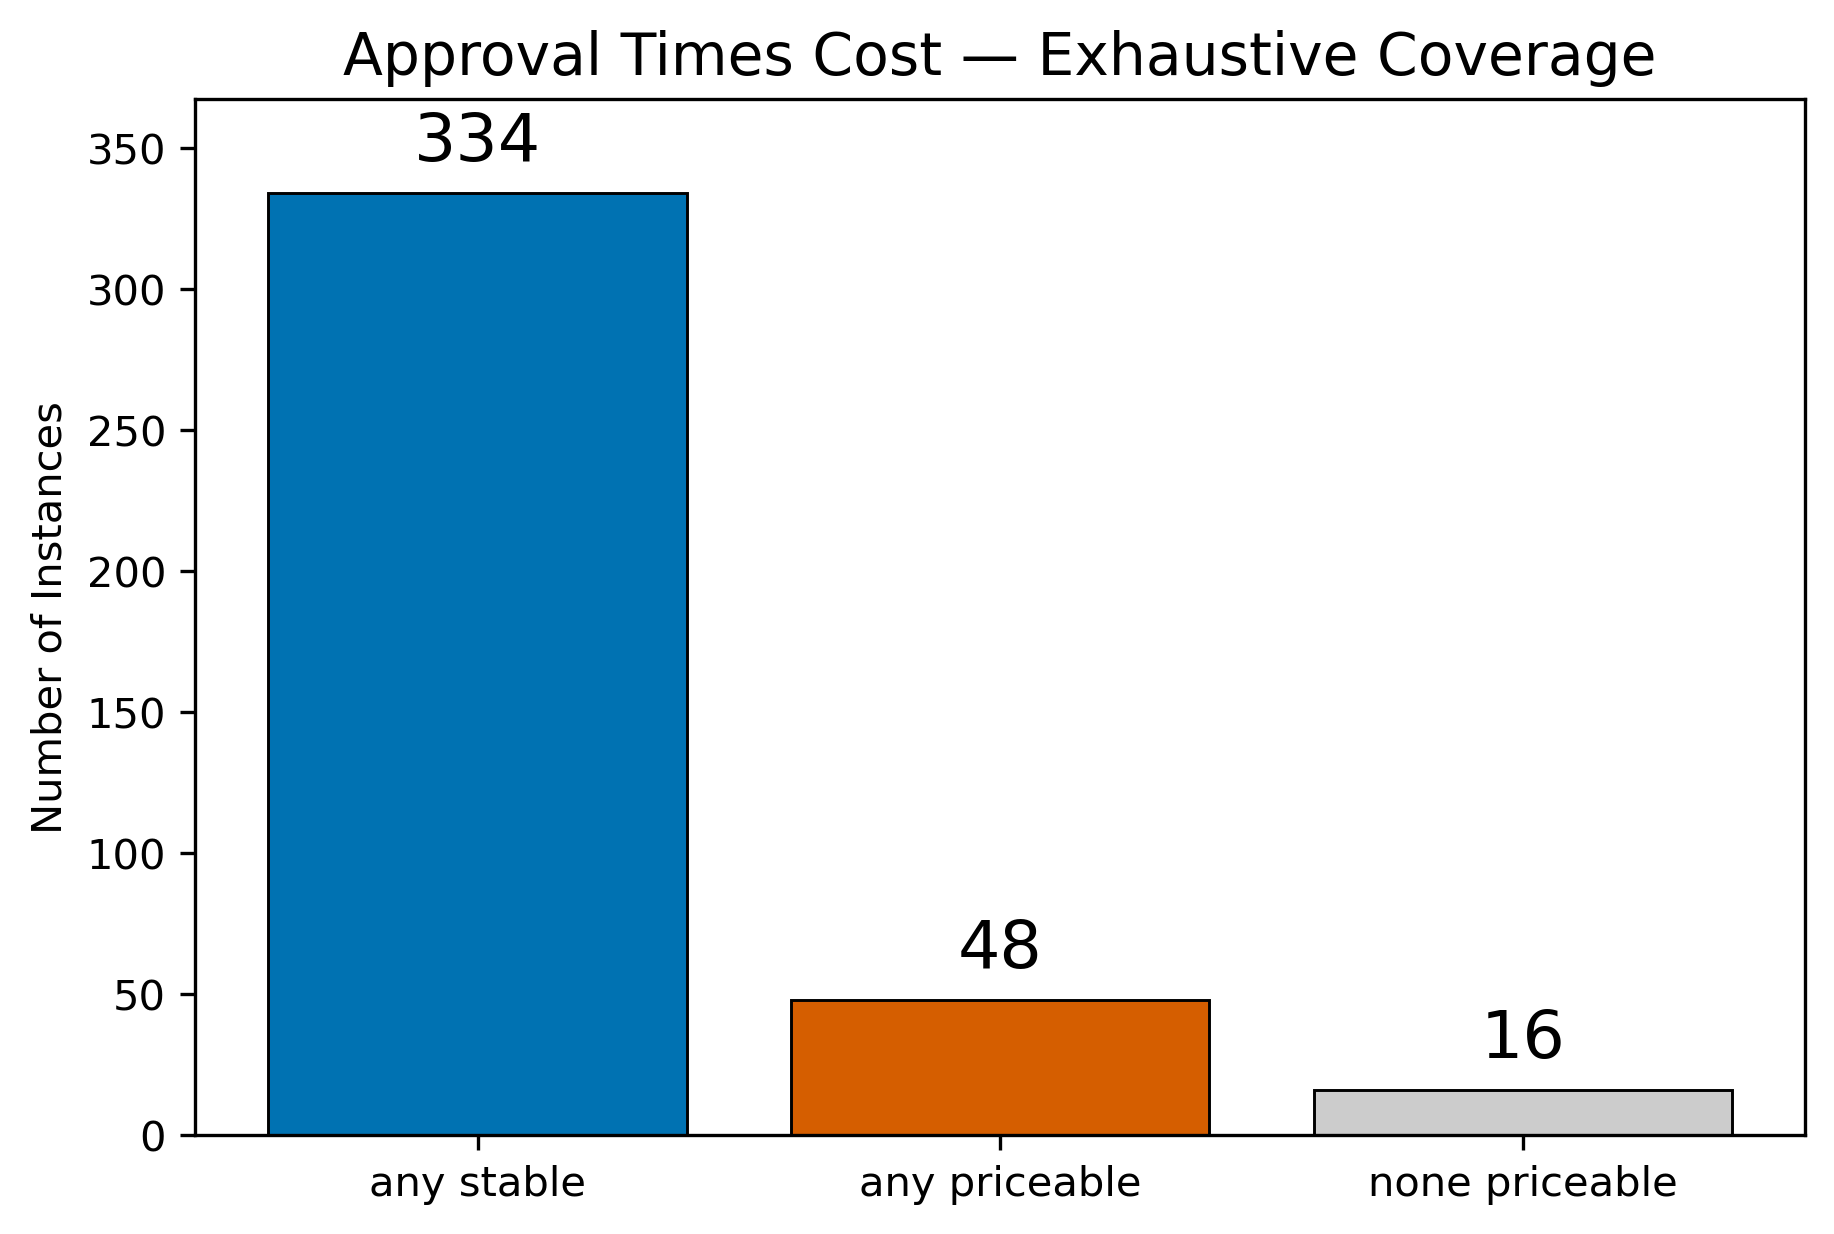
\includegraphics[width=0.7\textwidth]{figures/plots/approval-times-cost/approval_times_cost_coverage_exhaustive.png}
  \caption{Number of instances of standard approval-based cost-adjusted elections, where at least one method return an exhaustive stable priceable or priceable allocation.}
  \label{fig:myplot}
\end{figure}
\begin{figure}[H]         
  \centering              
  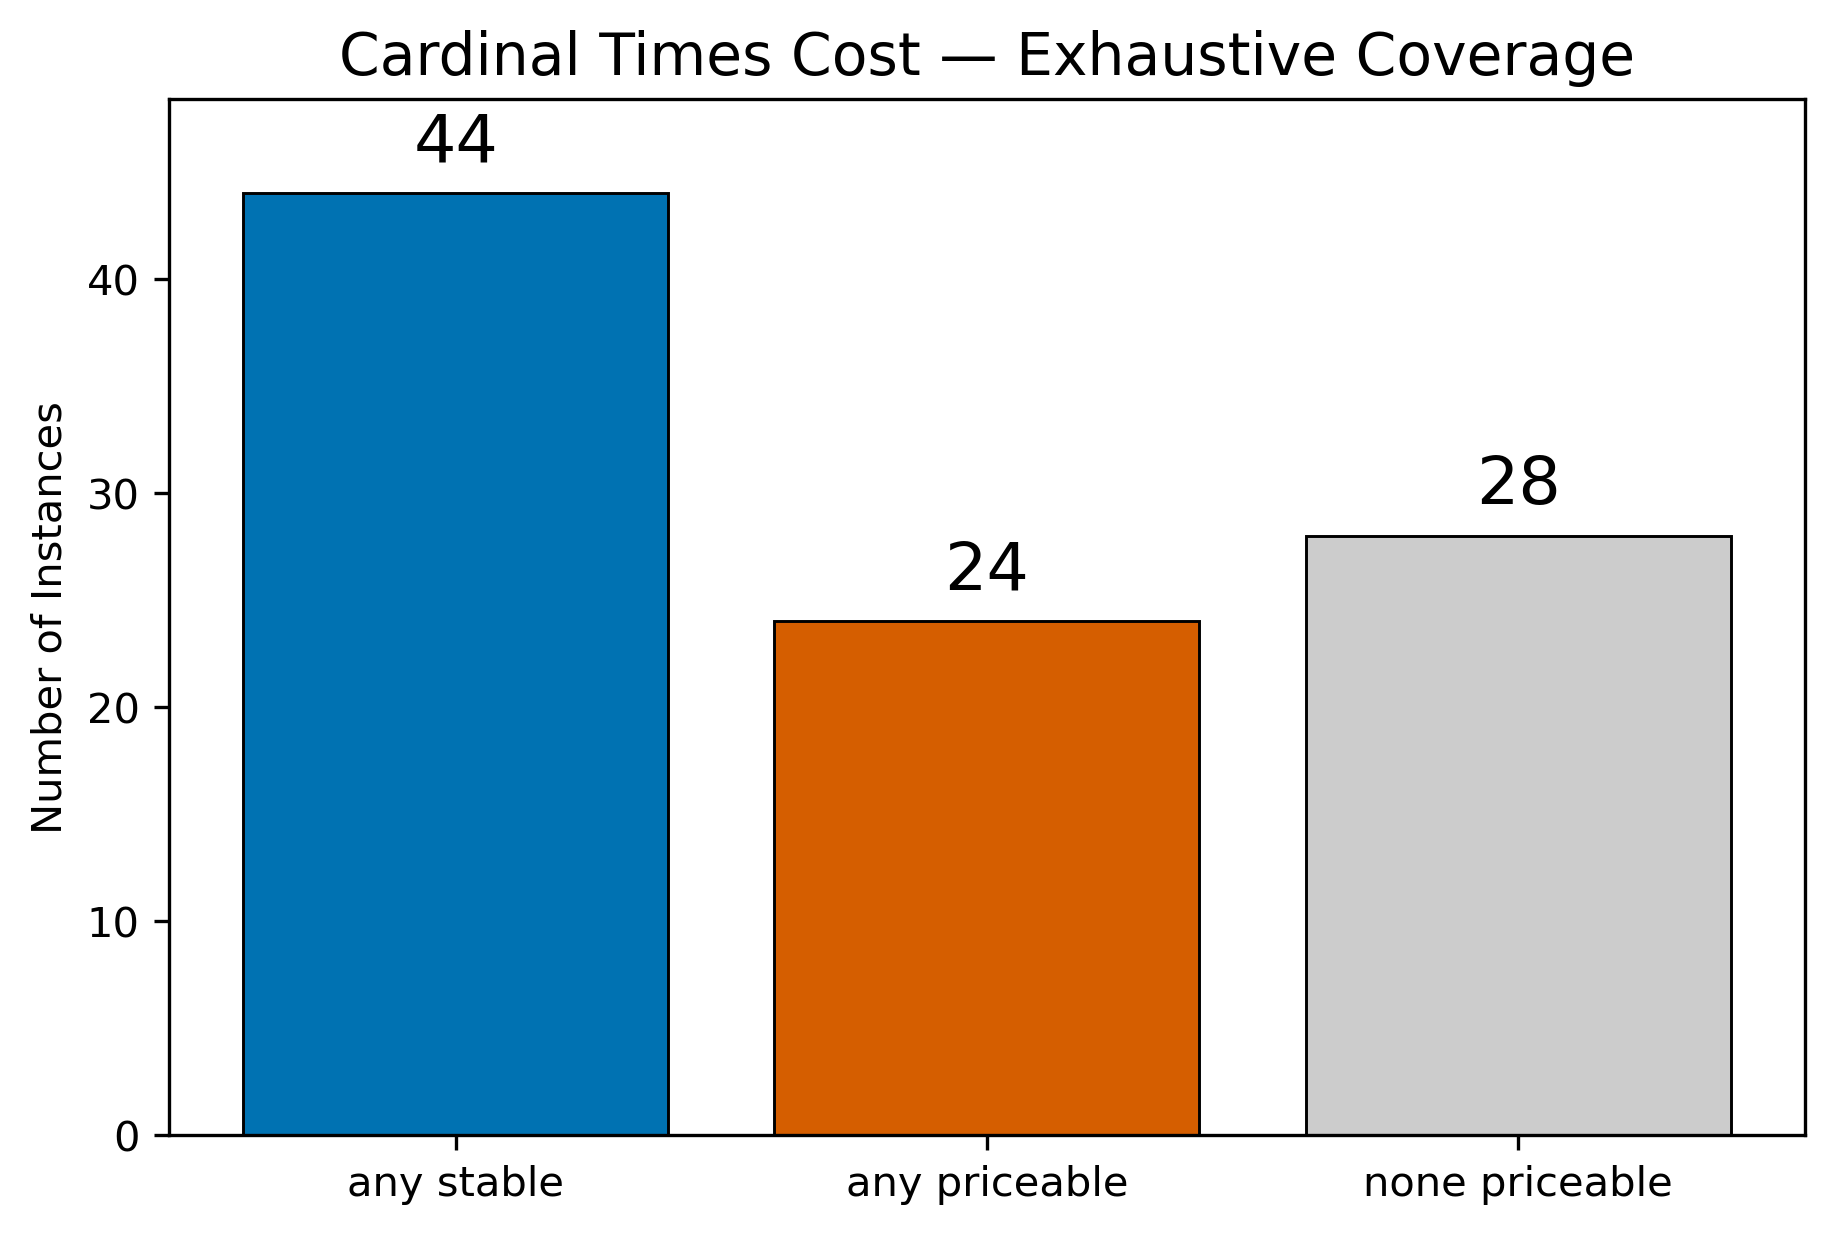
\includegraphics[width=0.7\textwidth]{figures/plots/cardinal-times-cost/cardinal_times_cost_coverage_exhaustive.png}
  \caption{Number of instances of standard cardinal-based cost-adjusted elections, where at least one method return an exhaustive stable priceable or priceable allocation.}  \label{fig:myplot}
\end{figure}
We observe that, again, the best results are by far for approval-based elections. There, at least $1$ method returns a perfect allocation in $83\%$ of elections, compared to only about $50\%$ for cardinal-based cases, regardless of the application of cost utility. All methods collectively tend to perform significantly worse when working with cardinal ballots.

However, it does not necessarily mean, that for the elections where none of the tested election rules provide exhaustive priceable or stable priceable elections, the election rules behave poorly. As we are aware of election instances, where no outcome is priceable while exhaustive, we check in how many cases the tested methods failed to find existing allocations satisfying the criteria. 
\begin{figure}[H]         
  \centering              
  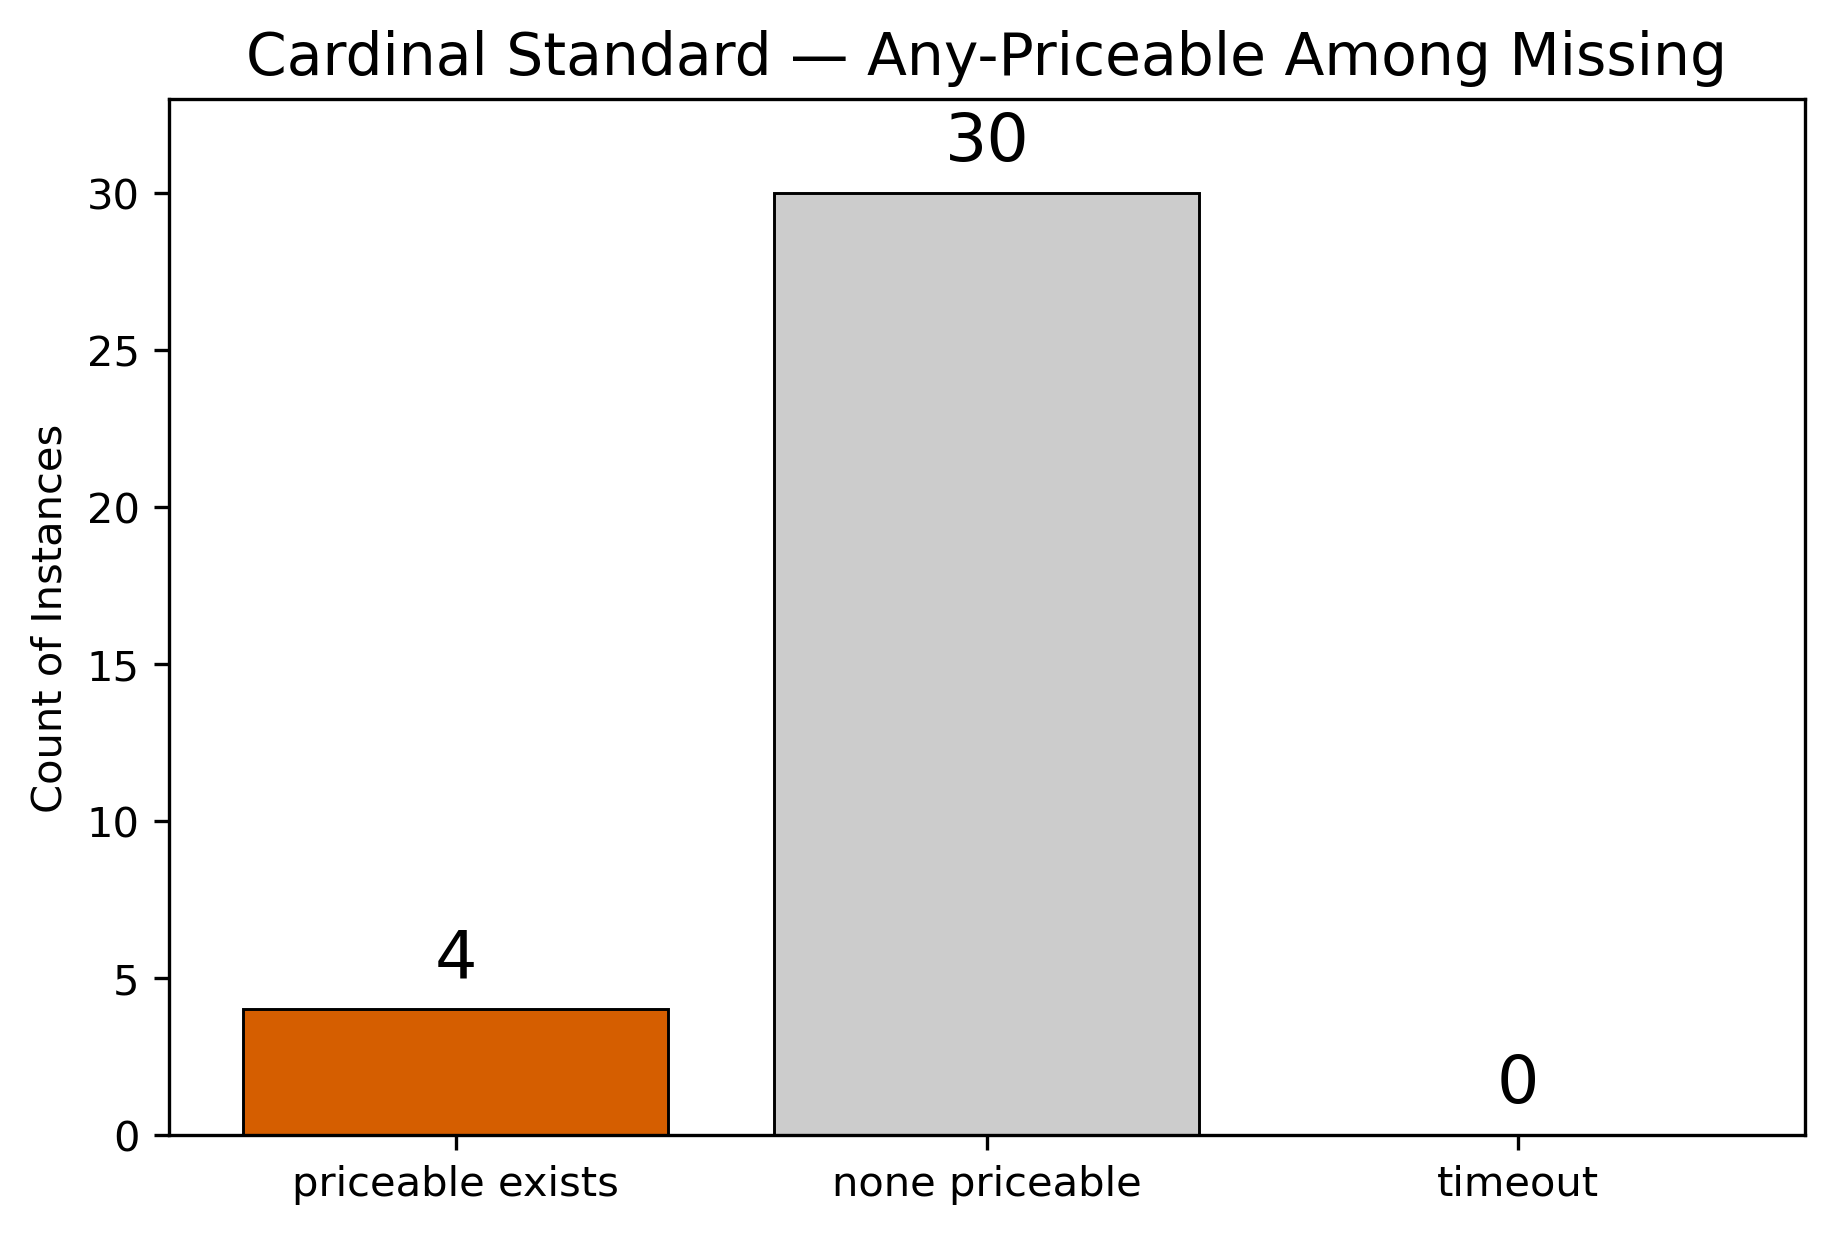
\includegraphics[width=0.7\textwidth]{figures/plots/cardinal-standard/cardinal_standard_any_priceable.png}
  \caption{Number of instances, for which no method found exhaustive priceable solution, where such solution a exists or does not, for cardinal-based elections with additive score utilities.}
  \label{fig:myplot}
\end{figure}
\begin{figure}[H]         
  \centering              
  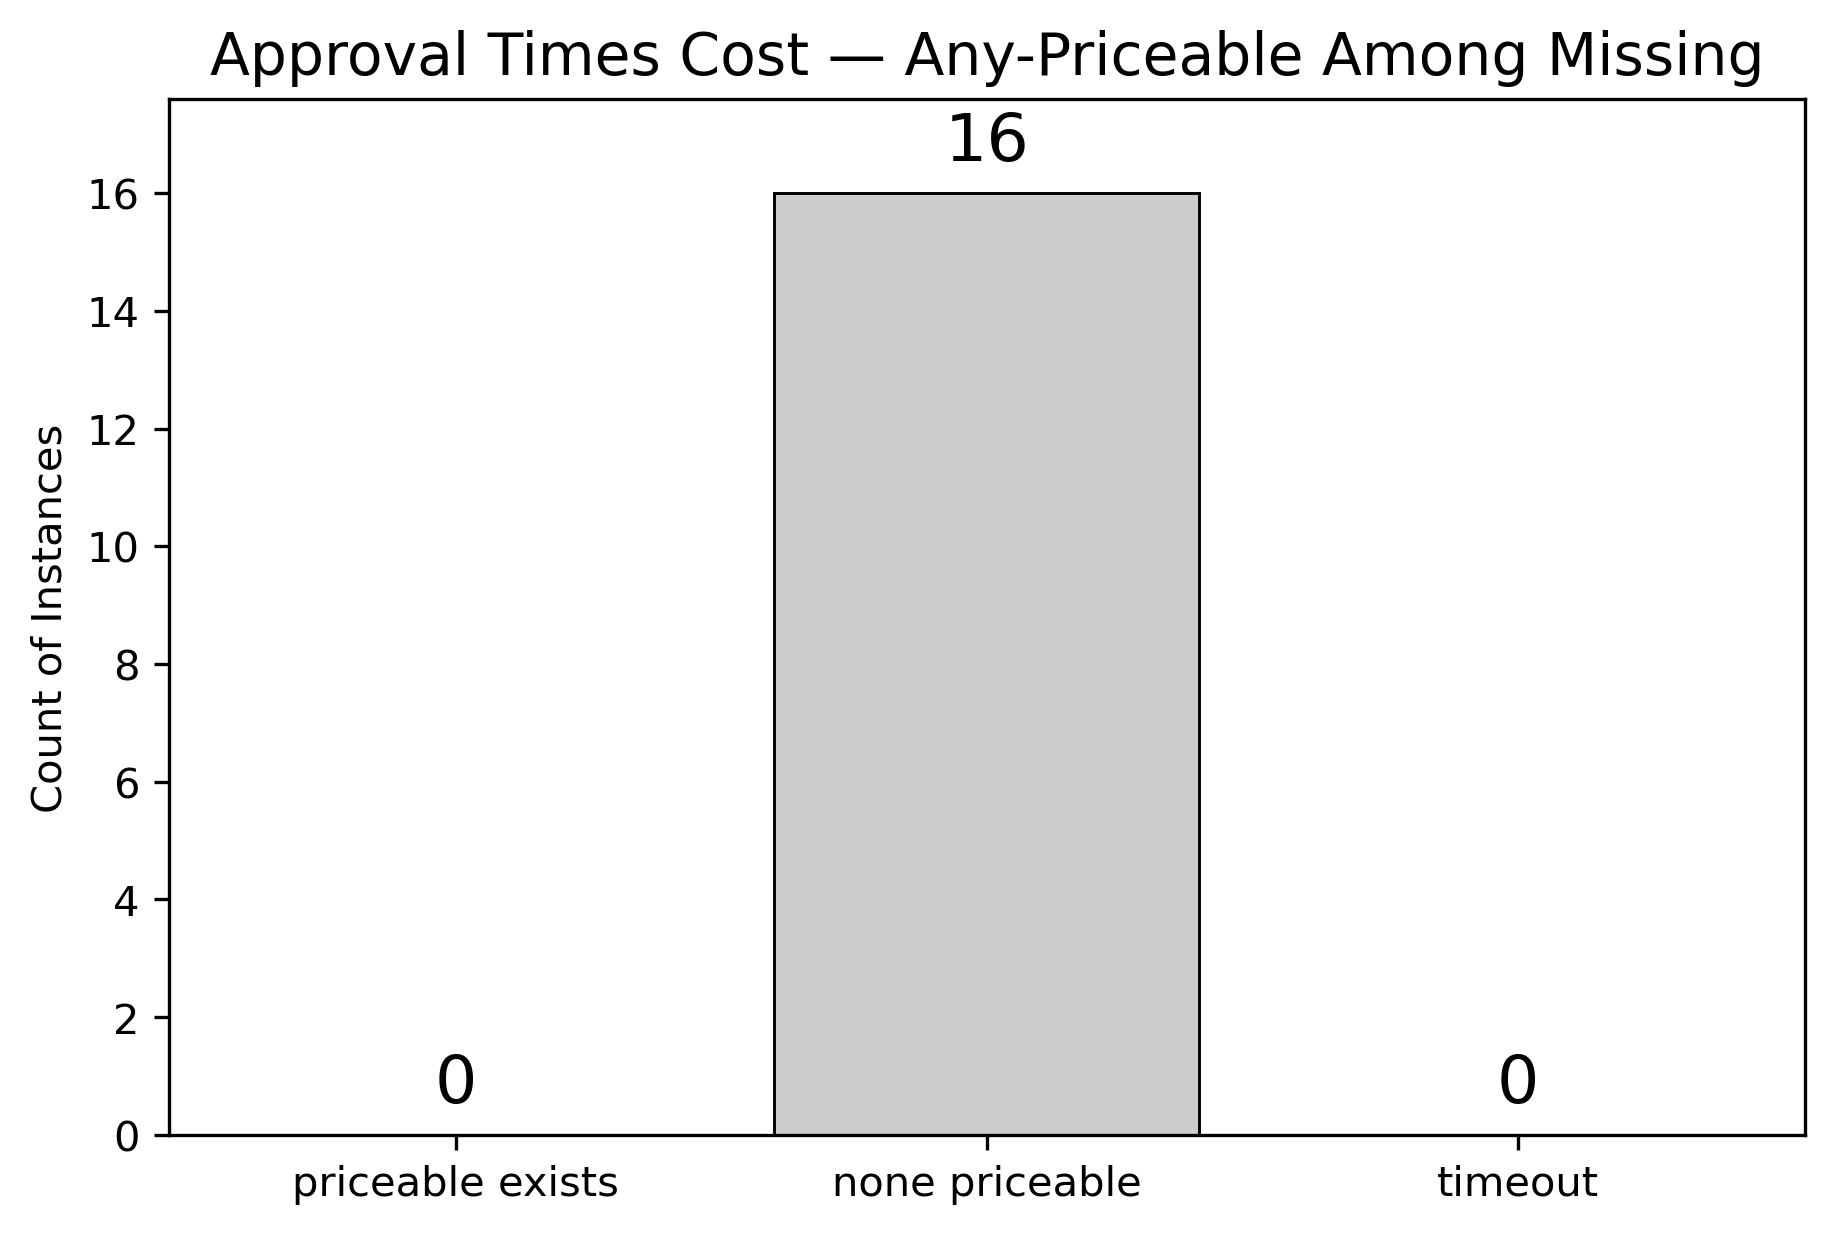
\includegraphics[width=0.7\textwidth]{figures/plots/approval-times-cost/approval_times_cost_any_priceable.png}
  \caption{Number of instances, for which no method found exhaustive priceable solution, where such a solution exists or does not, for approval-based elections with cost utilities.}
  \label{fig:myplot}
\end{figure}
\begin{figure}[H]         
  \centering              
  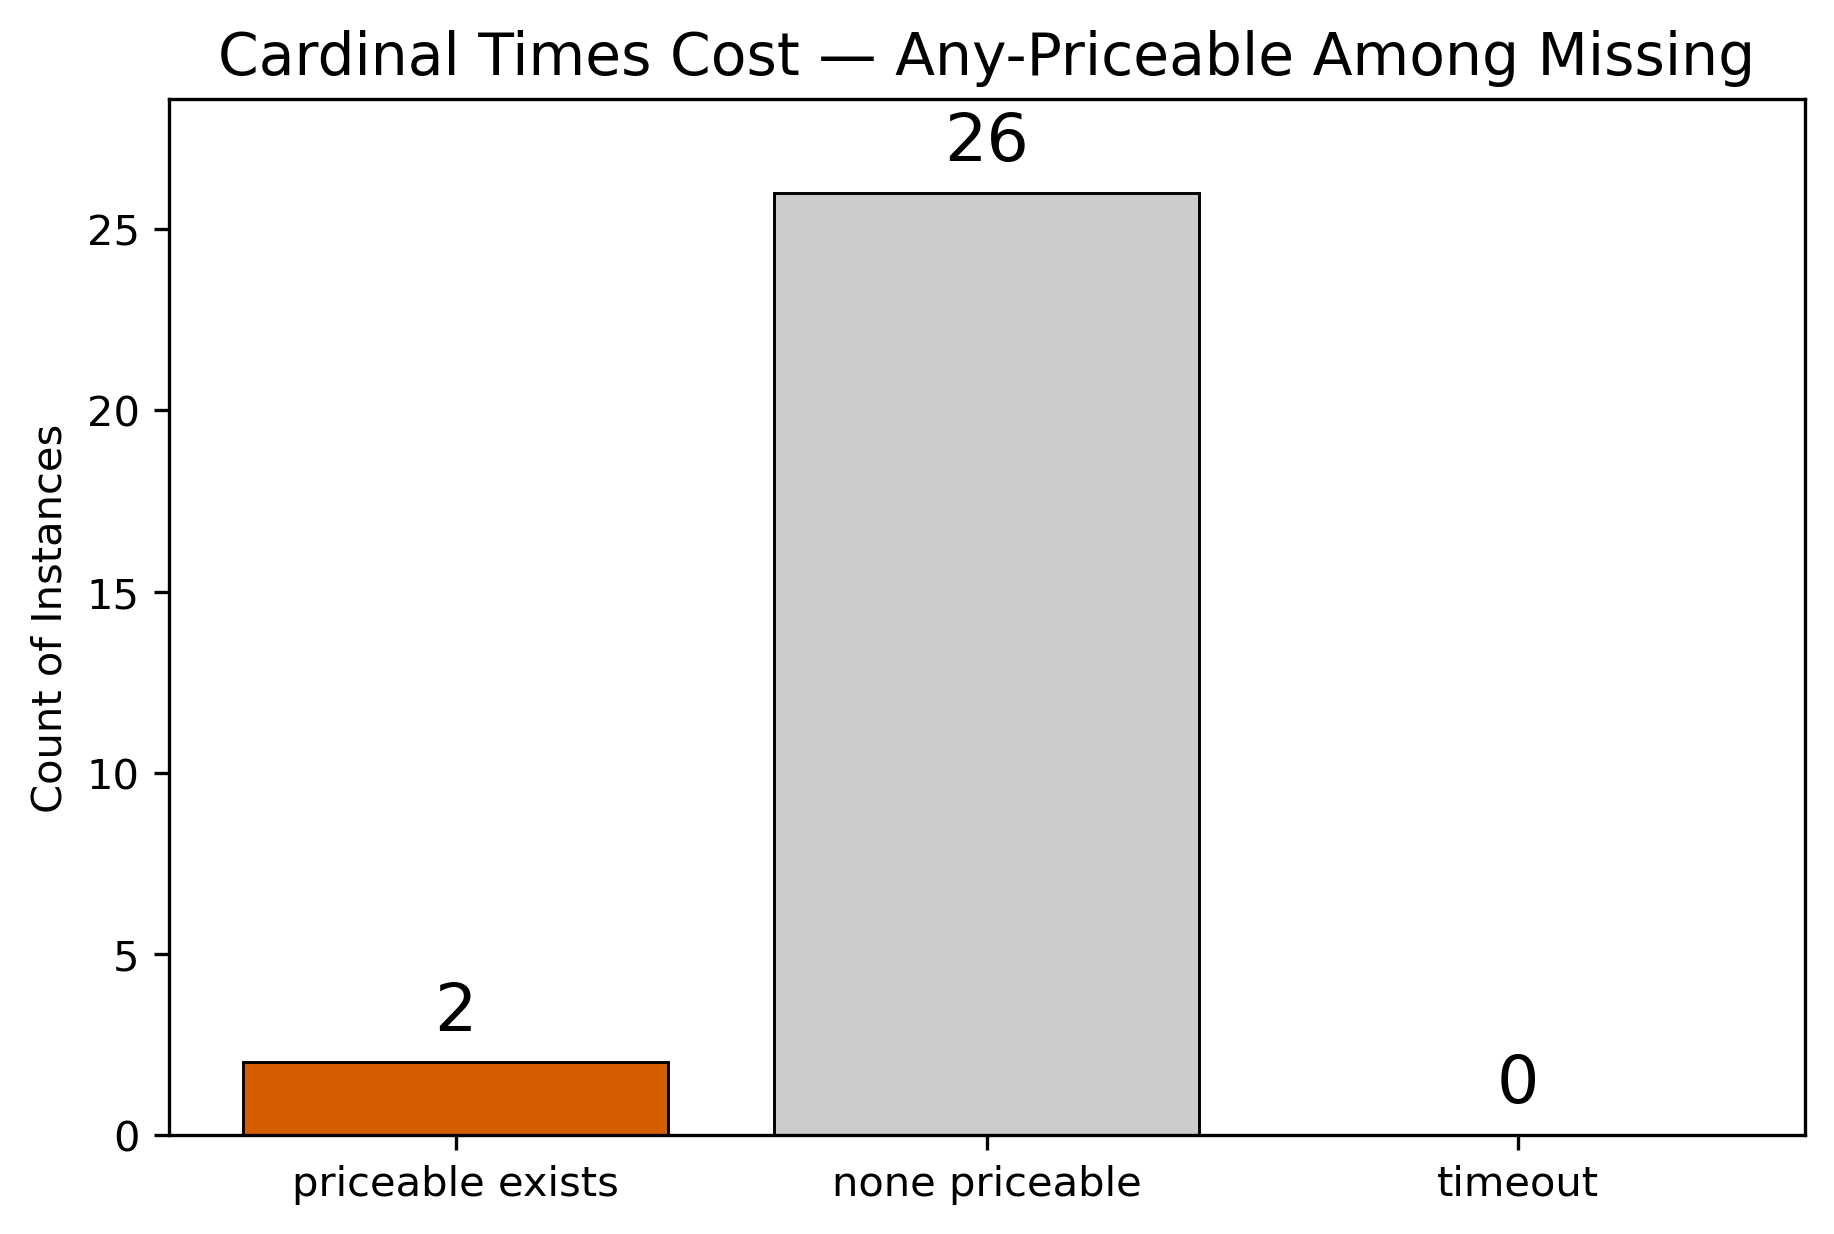
\includegraphics[width=0.7\textwidth]{figures/plots/cardinal-times-cost/cardinal_times_cost_any_priceable.png}
  \caption{Number of instances, for which no method found exhaustive priceable solution, where such a solution exists or does not, for cardinal-based elections with cost utilities.}
  \label{fig:myplot}
\end{figure}
It turns out, that depending on the election setting and satisfaction measure, in over $90\%$ of cases where no method has found an exhaustive priceable allocation, it was because such an allocation does not exist.

Finally, we do the same analysis, but for stable priceability. We check, among the instances where all methods failed to return a stable priceable and exhaustive allocation, how many of them actually have such a solution.
\begin{figure}[H]         
  \centering              
  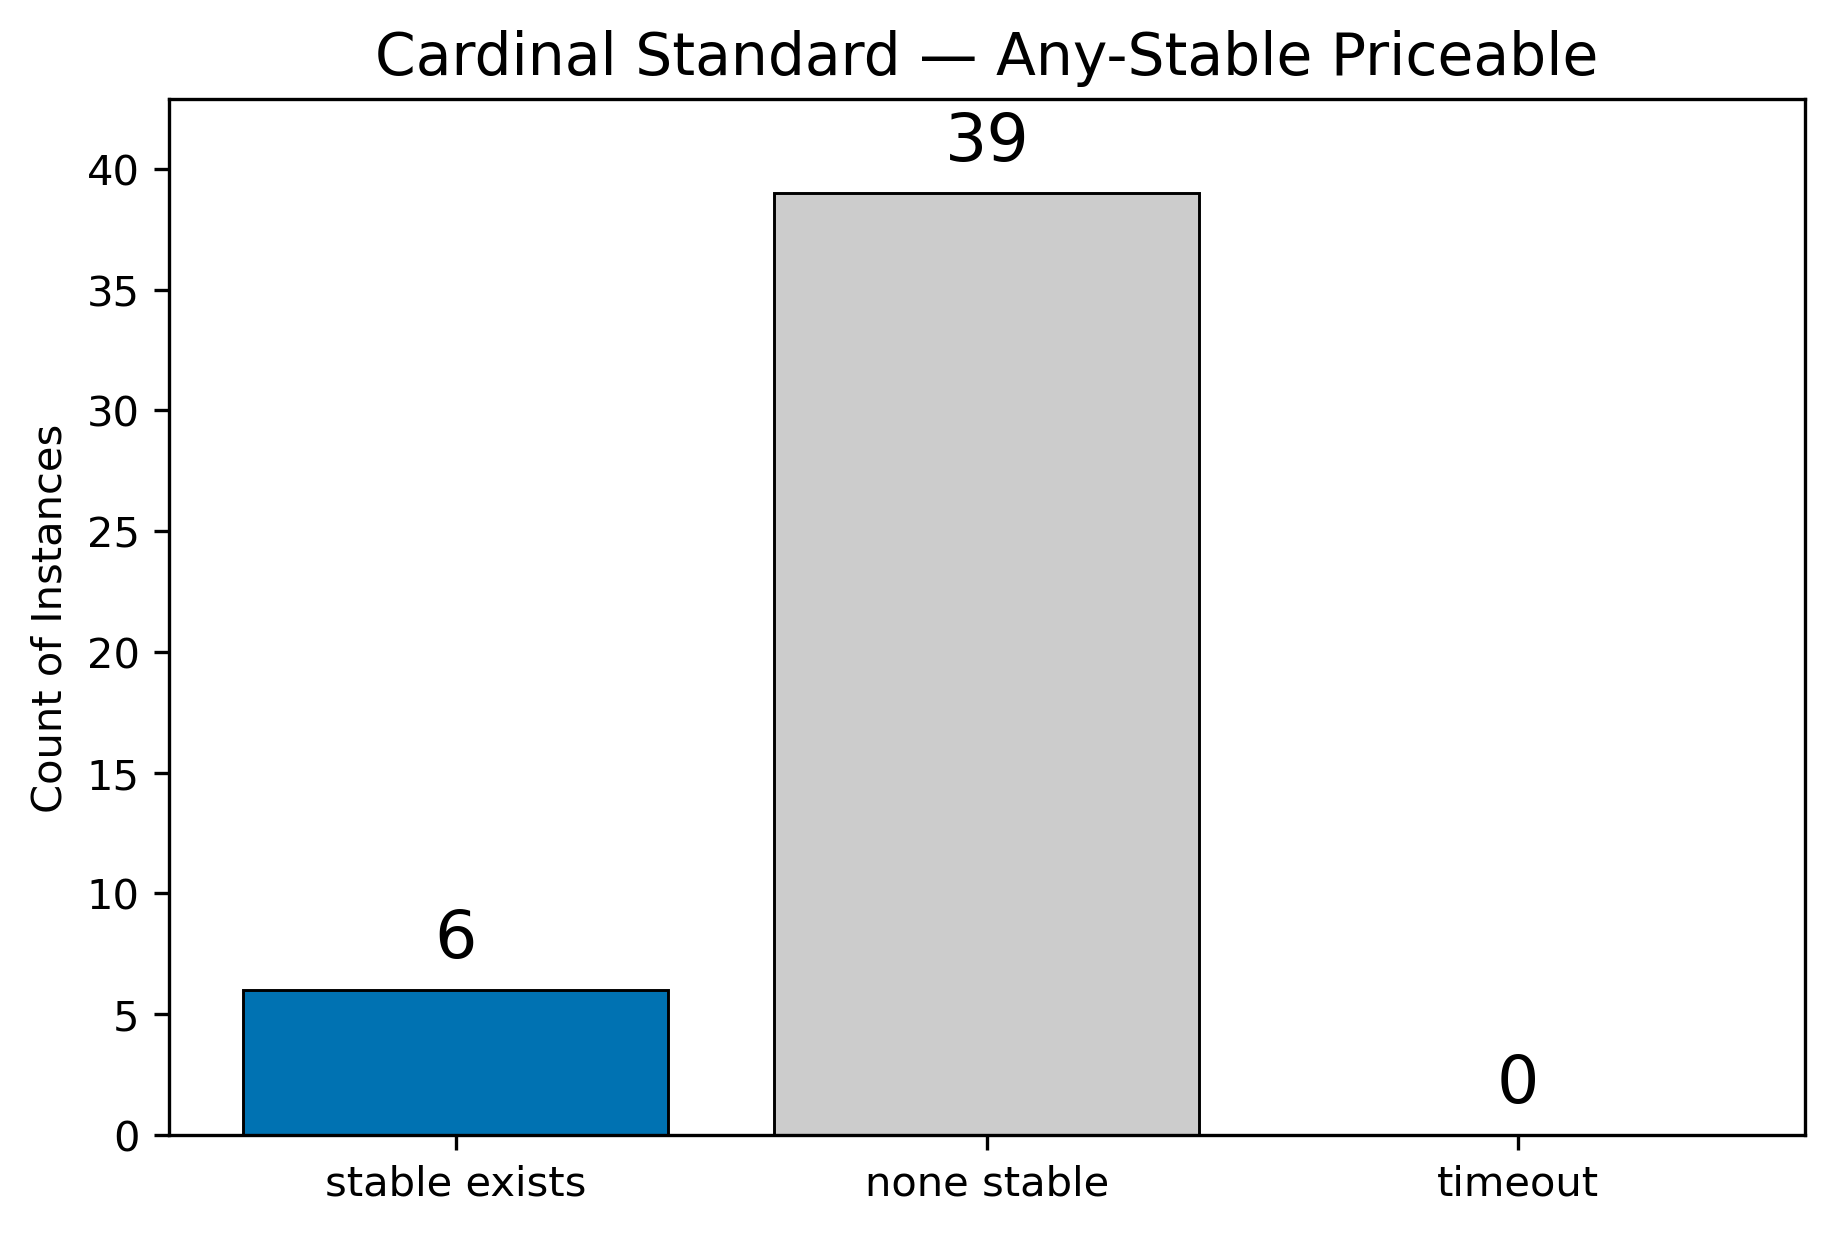
\includegraphics[width=0.7\textwidth]{figures/plots/cardinal-standard/cardinal_standard_any_stable_exhaustive.png}
  \caption{Number of instances, for which no method found exhaustive stable priceable solution, where such a solution exists or does not, for cardinal-based elections with additive score utilities.}
  \label{fig:myplot}
\end{figure}
\begin{figure}[H]         
  \centering              
  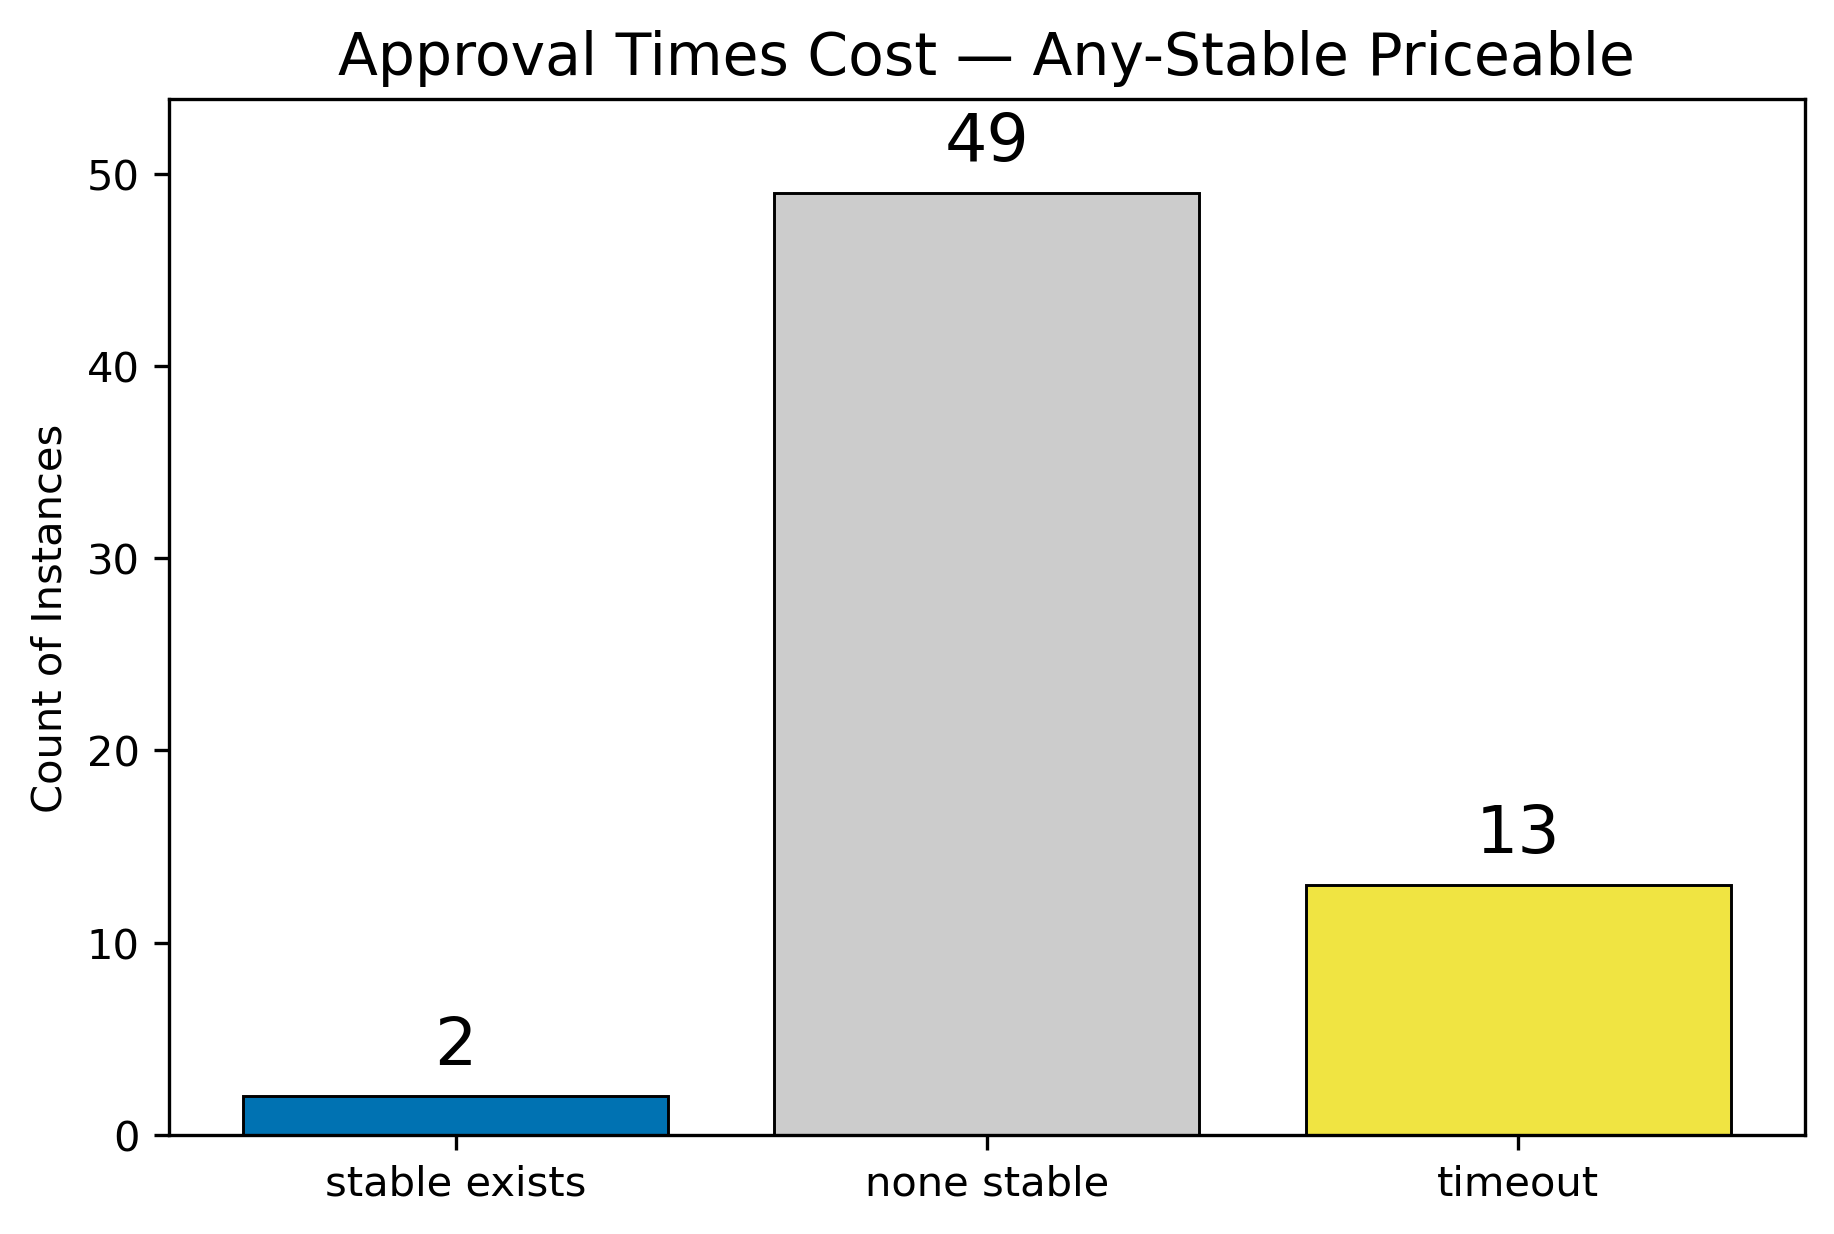
\includegraphics[width=0.7\textwidth]{figures/plots/approval-times-cost/approval_times_cost_any_stable_exhaustive.png}
  \caption{Number of instances, for which no method found exhaustive stable priceable solution, where such a solution exists or does not, for approval-based elections with cost utilities.}
  \label{fig:myplot}
\end{figure}
\begin{figure}[H]         
  \centering              
  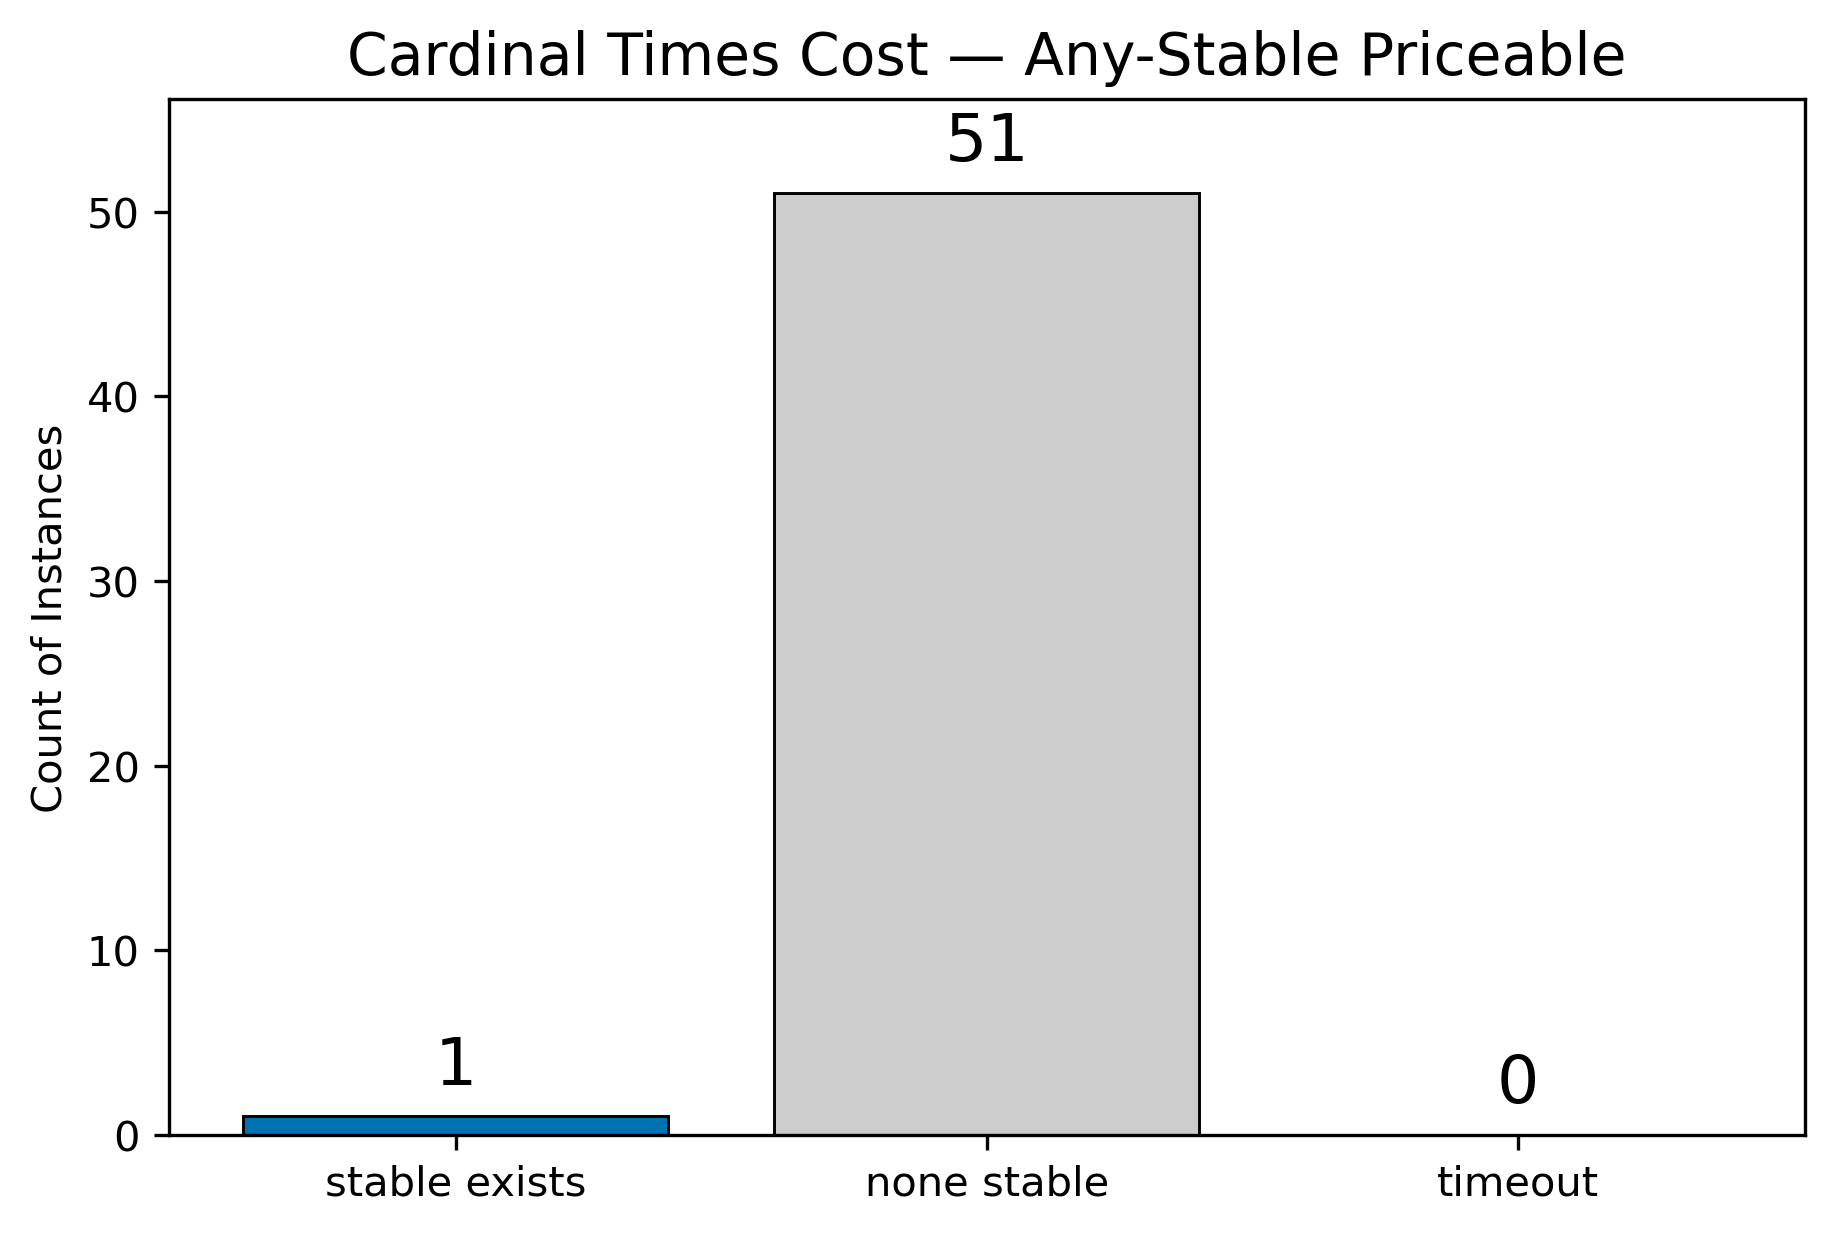
\includegraphics[width=0.7\textwidth]{figures/plots/cardinal-times-cost/cardinal_times_cost_any_stable_exhaustive.png}
  \caption{Number of instances, for which no method found exhaustive stable priceable solution, where such a solution exists or does not, for cardinal-based elections with cost utilities.}
  \label{fig:myplot}
\end{figure}
Similarly as for pure priceability, tested methods fail to find exhaustive stable priceable outcomes largely, because they do not exist. Again, that should be considered an acceptable result for proportionality provided by variations of MES, no matter the type of ballot or satisfaction measure.